\documentclass[11pt,a4paper]{report}

\usepackage{fontspec}
\setmainfont{Times New Roman}

\usepackage[a4paper,top=1in,bottom=1in,left=1in,right=1in]{geometry}
\usepackage{setspace}
\setstretch{1.2}

\usepackage{graphicx}
\usepackage{booktabs}
\usepackage{tabularx}
\usepackage{longtable}
\usepackage{amsmath}
\usepackage{amssymb}
\usepackage{caption}
\usepackage{subcaption}
\usepackage{fancyhdr}
\usepackage{titlesec}
\usepackage{hyperref}
\usepackage{microtype}
\usepackage{cite}
\usepackage{xcolor}

\hypersetup{
    colorlinks=true,
    linkcolor=black,
    citecolor=black,
    urlcolor=blue,
    pdftitle={India Air Quality Analysis and Next-Day AQI Forecasting},
    pdfauthor={Akshad Makhana, Shubham Pawar, Yash Kolhe, Pranav Hadole}
}

% Header and Footer
\pagestyle{fancy}
\fancyhf{}
\fancyhead[L]{\small\nouppercase{\leftmark}}
\fancyhead[R]{\small Next-Day AQI Forecasting}
\fancyfoot[C]{\thepage}
\renewcommand{\headrulewidth}{0.4pt}
\renewcommand{\footrulewidth}{0.4pt}

% Chapter and section heading styling
\titleformat{\chapter}[display]
  {\normalfont\bfseries\Large}
  {\filright\MakeUppercase{\chaptertitlename} \Huge\thechapter}
  {1ex}
  {\titlerule\vspace{1ex}\filright}
\titlespacing*{\chapter}{0pt}{10pt}{20pt}

\begin{document}

% -------------------------------------------------------------
% COVER PAGE
% -------------------------------------------------------------
\begin{titlepage}
    \centering
    \vspace*{0.5cm}
    
    
\includegraphics[width=0.65\textwidth]{college-logo.png}
    \vspace{0.8cm}
    
    {\Large \textbf{SANJIVANI UNIVERSITY, KOPARGAON}}\\[0.2cm]
    {\large \textbf{Department of Artificial Intelligence and Data Science}}\\[0.15cm]
    {\normalsize Academic Year 2026--2027 | Semester 5 (Third Year B.Tech)}\\[0.3cm]
    {\small Course Code: \textbf{24UADPC302} --- Predictive Modeling Using SPSS (IBM)}\\[1.2cm]
    
    \rule{\textwidth}{1.5pt}\\[0.4cm]
    {\huge \textbf{India Air Quality Analysis and}}\\[0.25cm]
    {\huge \textbf{Next-Day AQI Forecasting}}\\[0.3cm]
    {\large A Reproducible, Leak-Free Machine Learning Framework with TreeSHAP Interpretability and Conformal Uncertainty Quantification}\\[0.4cm]
    \rule{\textwidth}{1.5pt}\\[1.4cm]
    
    \begin{minipage}[t]{0.48\textwidth}
        \textbf{Submitted By:}\\[0.2cm]
        \begin{tabular}{ll}
            \textbf{Akshad Makhana} & (PRN: 2124UDSM1007) \\
            \textbf{Shubham Pawar}  & (PRN: 2124UDSM1074) \\
            \textbf{Yash Kolhe}     & (PRN: 2124UDSM1107) \\
            \textbf{Pranav Hadole}  & (PRN: 2124UDSM1108) \\
        \end{tabular}
    \end{minipage}
    \hfill
    \begin{minipage}[t]{0.45\textwidth}
        \flushright
        \textbf{Under the Guidance of:}\\[0.2cm]
        \textbf{Mr. Rohit Pawar}\\[0.1cm]
        Assistant Professor\\
        Department of AI \& Data Science\\
        Sanjivani University, Kopargaon
    \end{minipage}
    
    \vfill
    {\large Kopargaon, Maharashtra, India}\\[0.1cm]
    {\small October 2026}
\end{titlepage}

% -------------------------------------------------------------
% PRELIMINARY PAGES
% -------------------------------------------------------------
\pagenumbering{roman}

\chapter*{Abstract}
\addcontentsline{toc}{chapter}{Abstract}
Ambient air pollution poses a grave public health risk across the Indian subcontinent, contributing to over 1.6 million premature annual mortalities. Although the Central Pollution Control Board (CPCB) operates continuous ambient air quality monitoring stations (CAAQMS) across major urban centers, deploying reliable next-day forecasting models is severely impeded by pervasive data missingness, seasonal volatility, localized sensor saturation, and subtle forms of temporal target leakage. This investigation delivers an end-to-end, scientifically defensible machine learning pipeline designed to predict composite continuous next-day Air Quality Index ($\text{AQI}_{t+1}$) across 18 major Indian municipal air sheds.

Using multi-year CAAQMS telemetry (2015--2020), we enforce a strict temporal barrier isolating historical training data ($\le \text{June 30, 2018}$), designated validation calibration ($N=2,982$, July--December 2018), held-out primary test evaluation ($N=6,201$, 2019), and an exogenous shock stress test ($N=3,124$, 2020 COVID-19 lockdown). Features include autoregressive lags ($t, t-1, t-6$), combustion precursor ratios ($\text{PM}_{2.5} / \text{PM}_{10}$), backward-looking rolling moments, and deterministic circular calendar harmonics ($\sin, \cos$ day-of-year on a 365.25-day cycle). In chronological cross-validation, a tuned Random Forest Regressor ($n=100$, $\text{max\_depth}=10$, $\text{min\_samples\_split}=5$) was selected as champion over Ridge Regression and HistGradientBoosting based on pre-declared validation MAE.

On the 2019 held-out test cohort, the champion Random Forest achieved a Mean Absolute Error of \textbf{26.30 AQI points} (+15.28\% error reduction over Naive Persistence at 31.04), a Root Mean Squared Error of \textbf{55.62} (+20.81\% error reduction), and an $R^2$ of \textbf{0.8398}. Operational CPCB category diagnostic accuracy reached \textbf{74.36\%}. Under the 2020 lockdown shock, the pipeline demonstrated sustained generalization with an MAE of \textbf{19.33} (+10.64\% improvement). A comprehensive sensitivity audit revealed that localized sensor saturation in Ahmedabad contributed 72.59\% of total network squared error; excluding Ahmedabad reduced network RMSE to \textbf{29.97 AQI points} ($R^2 = 0.8931$).

Model interpretability was formalized via Path-Dependent TreeSHAP, verifying that $\text{AQI}_t$ and $\text{PM}_{2.5}$ provide 66.8\% of global attribution, while additive reconstructions matched direct predictions within $5.91 \times 10^{-12}$ AQI points. Conformal prediction intervals were calibrated on pre-2019 validation residuals, yielding finite-sample margins of $\pm 57.06$ (90\%) and $\pm 90.38$ (95\%) AQI points, attaining 90.21\% and 94.97\% empirical test coverage. Finally, a robust inference command-line interface was developed with schema validation, non-negativity checks, transparent training-median disclosure, and unknown-city extrapolation warnings. All source code, serialized models, evaluation CSVs, and an 88-test regression suite are permanently preserved for peer verification.

\vspace{0.8cm}
\noindent \textbf{Keywords:} Air Quality Index (AQI), Next-Day Forecasting, Machine Learning, Random Forest, Temporal Data Leakage, TreeSHAP, Conformal Prediction, CAAQMS, Environmental Intelligence.

\clearpage

\tableofcontents
\clearpage

\listoffigures
\clearpage

\listoftables
\clearpage

% -------------------------------------------------------------
% MAIN BODY
% -------------------------------------------------------------
\pagenumbering{arabic}

\chapter{Introduction and Background}

\section{The Urban Air Pollution Crisis in India}
Ambient air pollution represents one of the most critical public health, environmental, and socio-economic emergencies facing modern India. Rapid urban development, intensive vehicular density, industrial manufacturing, regional biomass burning, and seasonal meteorological thermal inversions converge to generate prolonged episodes of hazardous atmospheric contamination \cite{who2021air}. Epidemiological assessments conducted by the World Health Organization and the Global Burden of Disease consortium estimate that chronic exposure to ambient fine particulate matter ($\text{PM}_{2.5}$) and gaseous combustion byproducts ($\text{NO}_2$, $\text{SO}_2$, $\text{CO}$, $\text{O}_3$) accounts for more than 1.6 million premature annual deaths across India.

To monitor atmospheric degradation and communicate health advisories, the Central Pollution Control Board (CPCB) formulated the National Air Quality Index (AQI) framework \cite{cpcb2014national}. The statutory CPCB index maps continuous precursor concentrations into an aggregated numerical scale spanning 0 to 500, partitioned into six statutory health hazard categories: Good ($0$--$50$), Satisfactory ($51$--$100$), Moderate ($101$--$200$), Poor ($201$--$300$), Very Poor ($301$--$400$), and Severe ($>400$).

\section{Challenges in Environmental Telemetry}
While the CPCB has expanded its Continuous Ambient Air Quality Monitoring Station (CAAQMS) network across more than 200 stations nationwide, raw observational records exhibit acute analytical hurdles:
\begin{enumerate}
    \item \textbf{High Missingness Rates and Sensor Dropouts:} CAAQMS surface analyzers experience periodic power interruptions, calibration downtime, and transmission dropouts, yielding missingness rates between 15\% and 60\% across primary criteria pollutants.
    \item \textbf{Atmospheric Non-Stationarity and Seasonal Inversions:} Indian meteorology is characterized by drastic seasonal shifts. Monsoon rains scavenge particulate matter, while winter atmospheric stagnation traps emissions within the planetary boundary layer, producing non-stationary statistical distributions.
    \item \textbf{Pervasive Temporal Data Leakage in Literature:} Academic literature frequently applies random train-test splitting or uses contemporaneous same-day predictor inputs to predict same-day AQI ($y_t = f(X_t)$). Such formulations conceal future temporal information, producing artificially inflated accuracy metrics that completely fail when deployed for genuine prospective forecasting.
    \item \textbf{Omission of Naive Baselines:} Complex deep learning and non-linear regression models are often promoted without demonstrating that they outperform a simple, cost-free Naive Persistence baseline ($\widehat{y}_{t+1} = y_t$).
\end{enumerate}

\section{Project Objectives}
This academic project establishes a reproducible, scientifically defensible machine learning framework for forecasting next-day city-level AQI ($\text{AQI}_{t+1}$) across 18 qualified Indian urban centers. The specific research objectives comprise:
\begin{enumerate}
    \item \textbf{Leakage-Free Feature Engineering:} Construct a temporal feature matrix relying strictly on information available at or before prediction origin day $t$, enforcing strict municipal boundary isolation.
    \item \textbf{Chronological Model Selection:} Benchmark multiple supervised candidate architectures against Naive Persistence across historical rolling folds ($\le \text{June 2018}$) and evaluate on a pre-declared designated validation period (July--December 2018).
    \item \textbf{Held-Out and Stress Evaluation:} Evaluate the frozen champion model on an untouched primary test set (calendar year 2019) and an exogenous stress-test partition (March--July 2020 COVID-19 lockdown).
    \item \textbf{Explainable AI (XAI):} Integrate Path-Dependent TreeSHAP to quantify global feature attributions and isolate individual prediction drivers.
    \item \textbf{Distribution-Free Uncertainty Quantification:} Formulate finite-sample split-conformal prediction intervals to supply decision-makers with rigorous probabilistic coverage bounds.
    \item \textbf{Production Deployment:} Deliver an audited, headless command-line interface (CLI) for prospective inference.
\end{enumerate}


\chapter{Data Provenance and Exploratory Data Analysis}

\section{Dataset Provenance and Architecture}
The empirical investigation utilizes the national air quality telemetry dataset compiled from CPCB CAAQMS surface stations and curated by Rohan Rao on Kaggle \cite{rao2020airquality}. The corpus spans January 1, 2015 through July 1, 2020 across 26 monitored Indian urban jurisdictions in 16 states and union territories. The raw telemetry consists of five primary relational tables:
\begin{itemize}
    \item \texttt{stations.csv}: Master metadata for 230 surface monitoring stations.
    \item \texttt{city\_day.csv}: 29,531 daily city-level observations (the primary modeling table).
    \item \texttt{city\_hour.csv}: 707,875 hourly city-level records.
    \item \texttt{station\_day.csv}: 108,035 station-level daily aggregations.
    \item \texttt{station\_hour.csv}: 2,589,083 station-level hourly records.
\end{itemize}
All raw datasets are permanently preserved with verified SHA-256 cryptographic checksums.

\section{Municipal Jurisdiction Qualification}
To eliminate spurious evaluations caused by fragmented monitoring histories, municipal eligibility was audited. Urban centers were classified based on observation density:
\begin{itemize}
    \item \textbf{Tier-1 Qualified (18 Cities):} Continuous multi-year telemetry with $>60\%$ valid daily records (Ahmedabad, Amaravati, Amritsar, Bengaluru, Brajrajnagar, Chennai, Delhi, Gurugram, Hyderabad, Jaipur, Jorapokhar, Kolkata, Lucknow, Mumbai, Patna, Talcher, Thiruvananthapuram, Visakhapatnam).
    \item \textbf{Tier-2 / Disqualified (8 Cities):} Stations installed late in 2019 or with $<40\%$ temporal coverage (e.g., Aizawl, Guwahati, Ernakulam, Coimbatore). These cities were quarantined to prevent historical distortion.
\end{itemize}

\section{Exploratory Data Analysis and Findings}
Figure~\ref{fig:eda_overview} summarizes national ambient AQI distribution dynamics, municipal disparities, seasonal patterns, and chemical precursor correlations.

\begin{figure}[htbp]
    \centering
    \begin{subfigure}[b]{0.48\textwidth}
        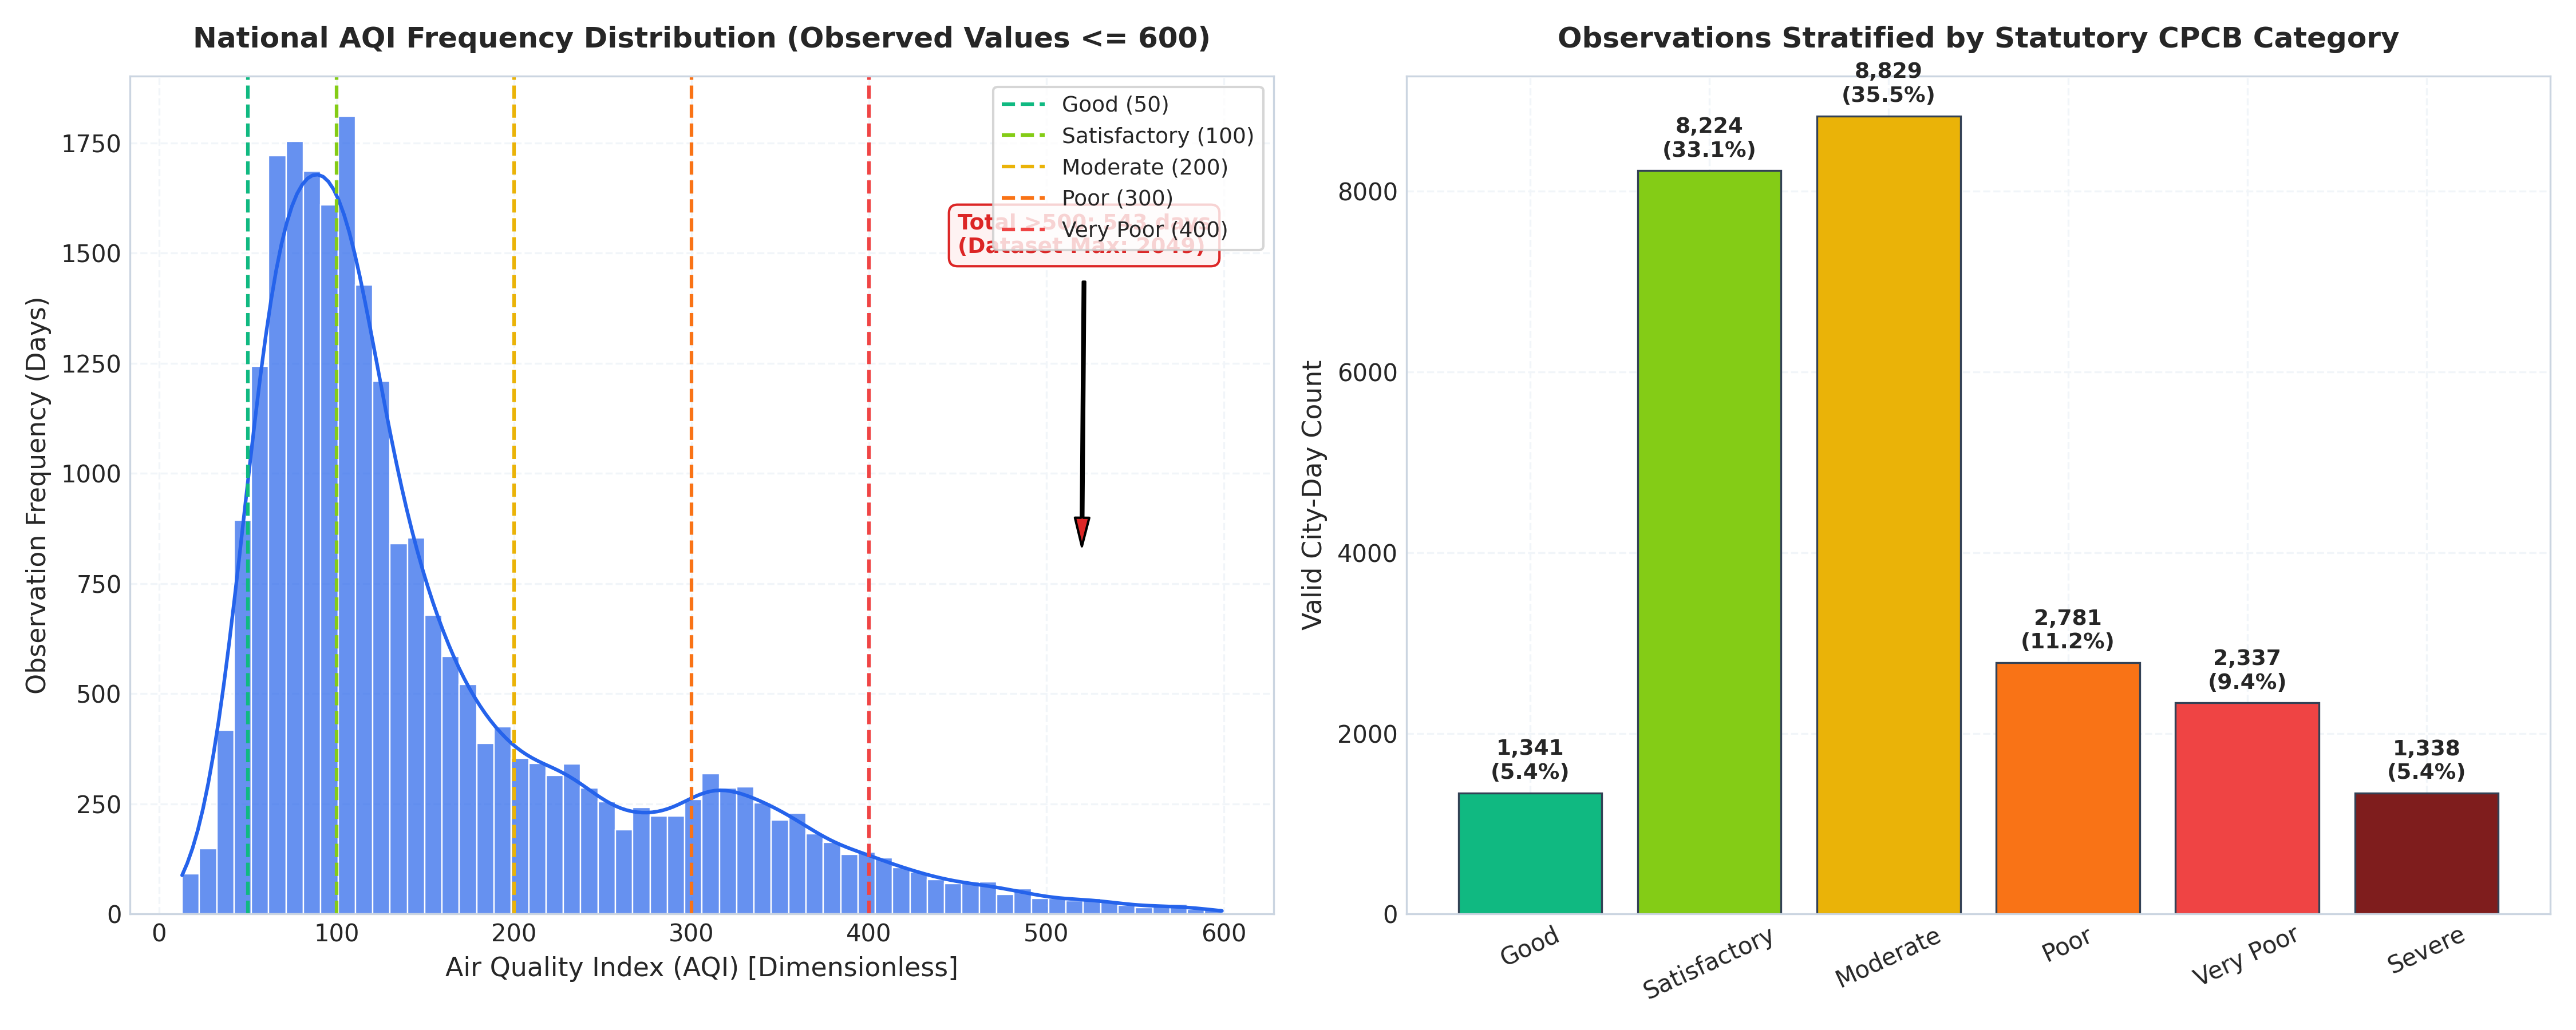
\includegraphics[width=\textwidth]{figures/01_aqi_distribution_and_cpcb_bands.png}
        \caption{National AQI Distribution and CPCB Tiers}
        \label{fig:dist}
    \end{subfigure}
    \hfill
    \begin{subfigure}[b]{0.48\textwidth}
        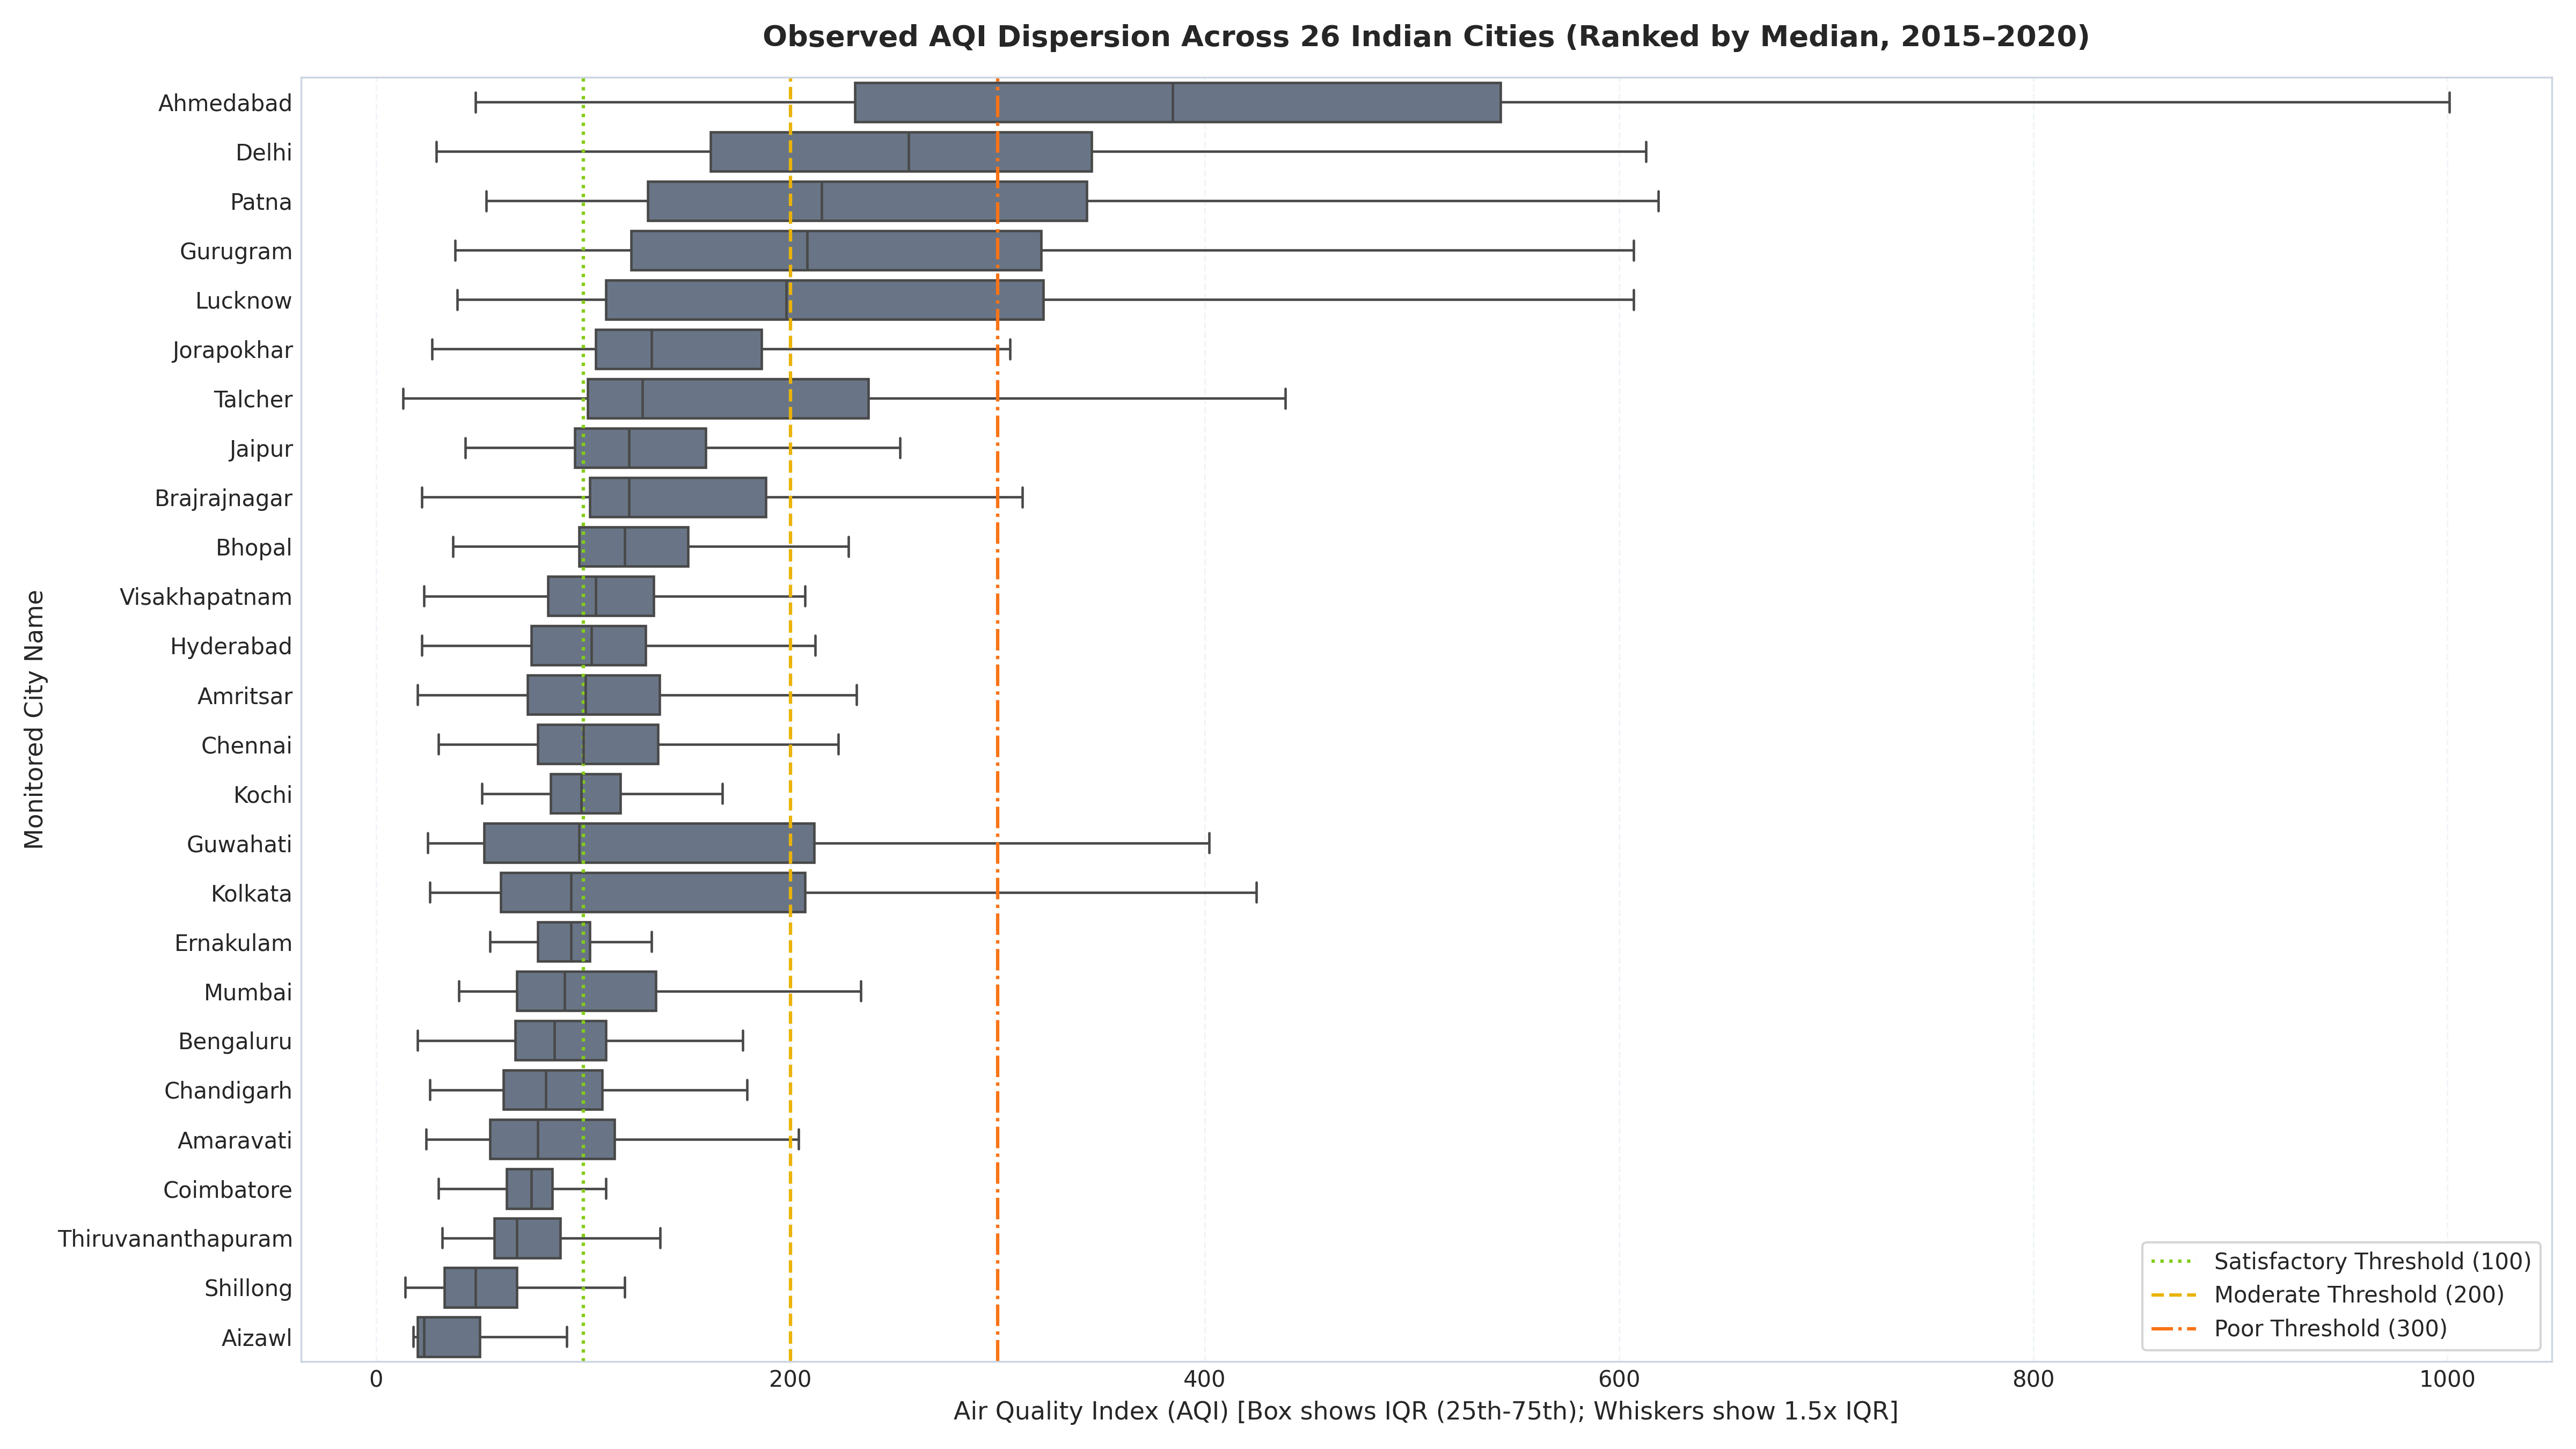
\includegraphics[width=\textwidth]{figures/02_city_level_aqi_comparison.png}
        \caption{Municipal AQI Disparities}
        \label{fig:cities}
    \end{subfigure}
    
    \vspace{0.4cm}
    \begin{subfigure}[b]{0.48\textwidth}
        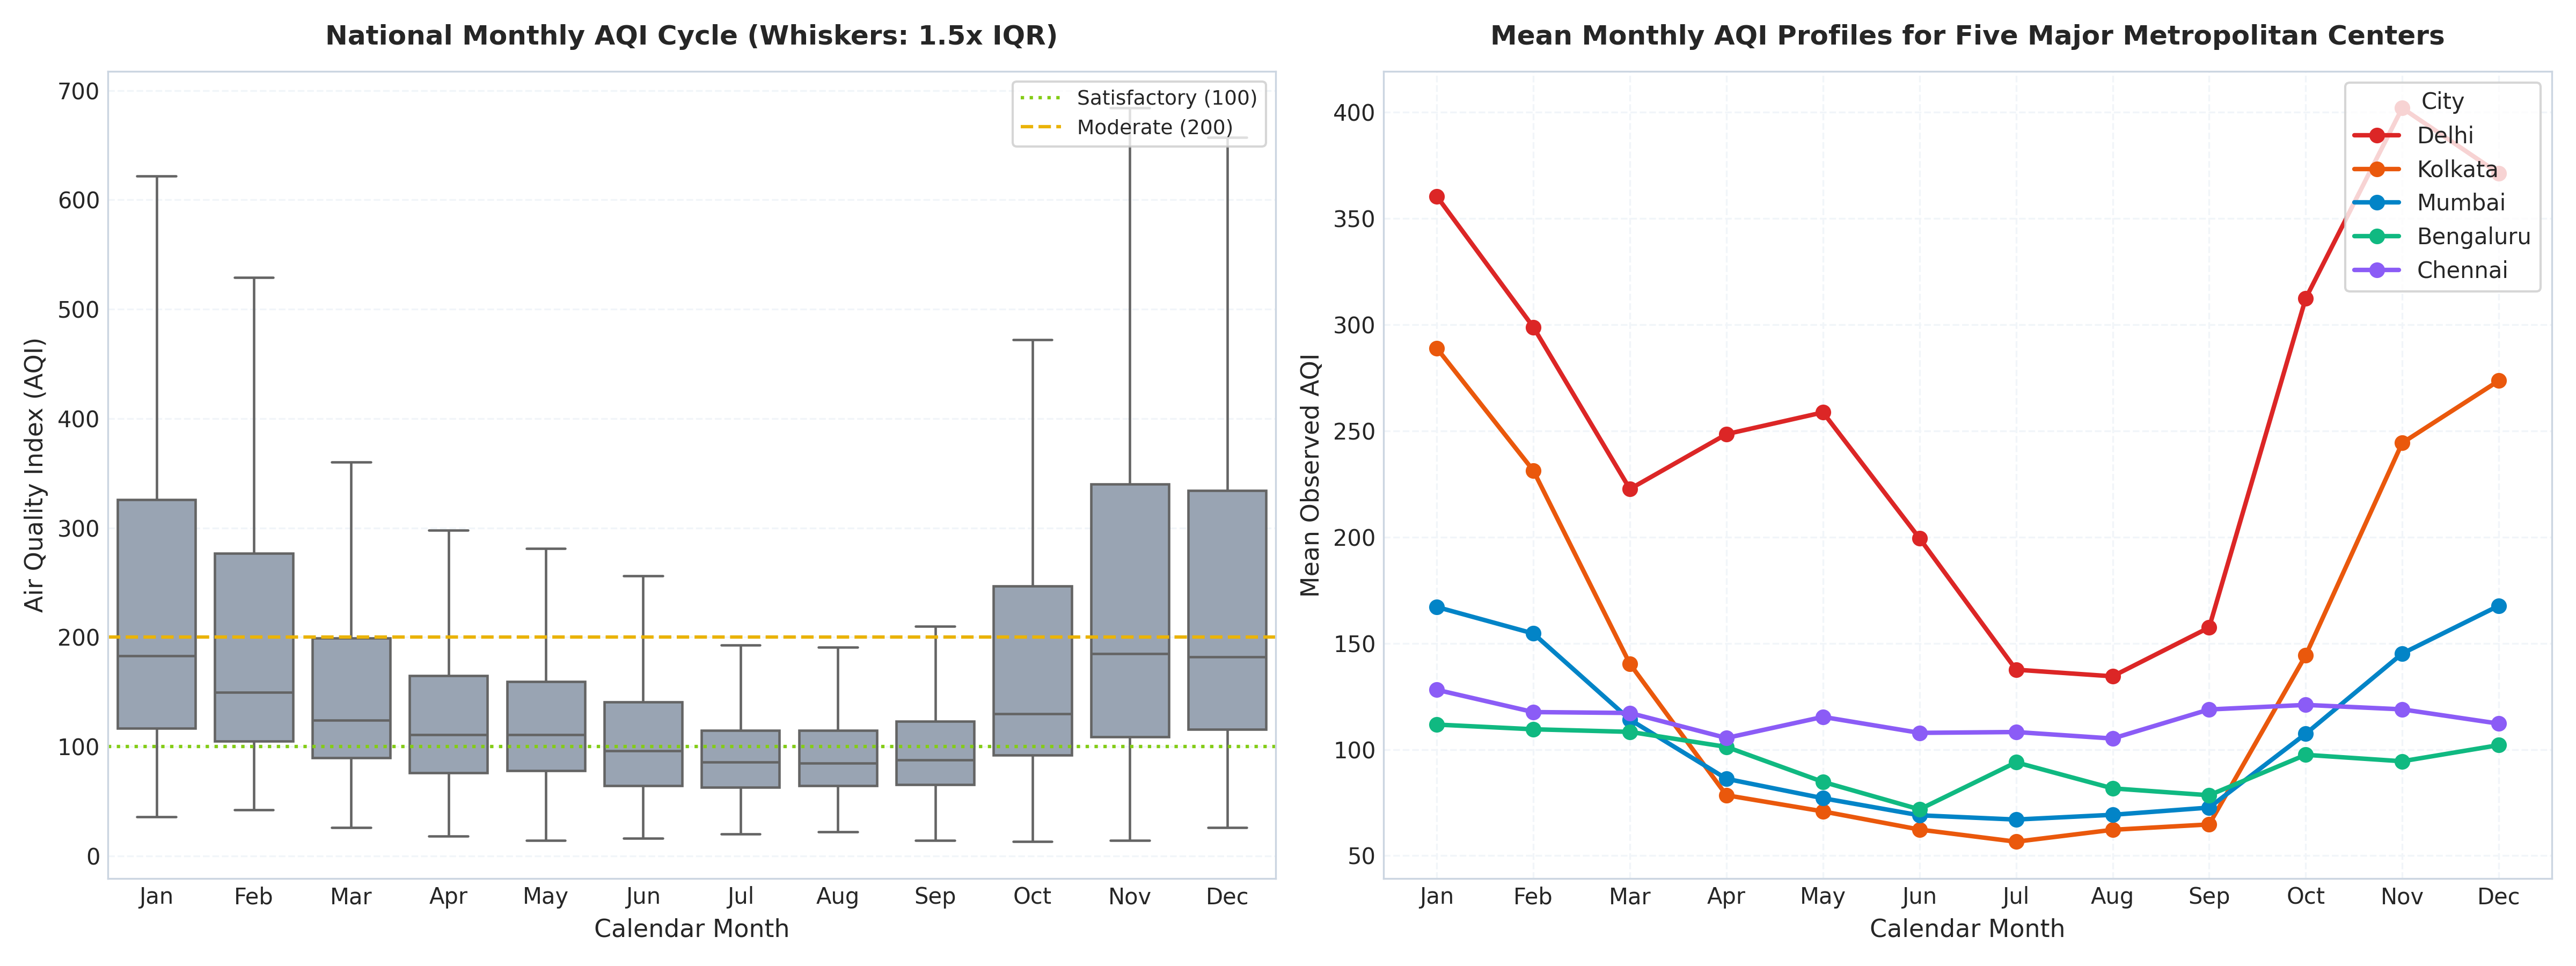
\includegraphics[width=\textwidth]{figures/03_seasonal_and_monthly_patterns.png}
        \caption{Seasonal Annual Cycle (Monsoon vs Winter)}
        \label{fig:season}
    \end{subfigure}
    \hfill
    \begin{subfigure}[b]{0.48\textwidth}
        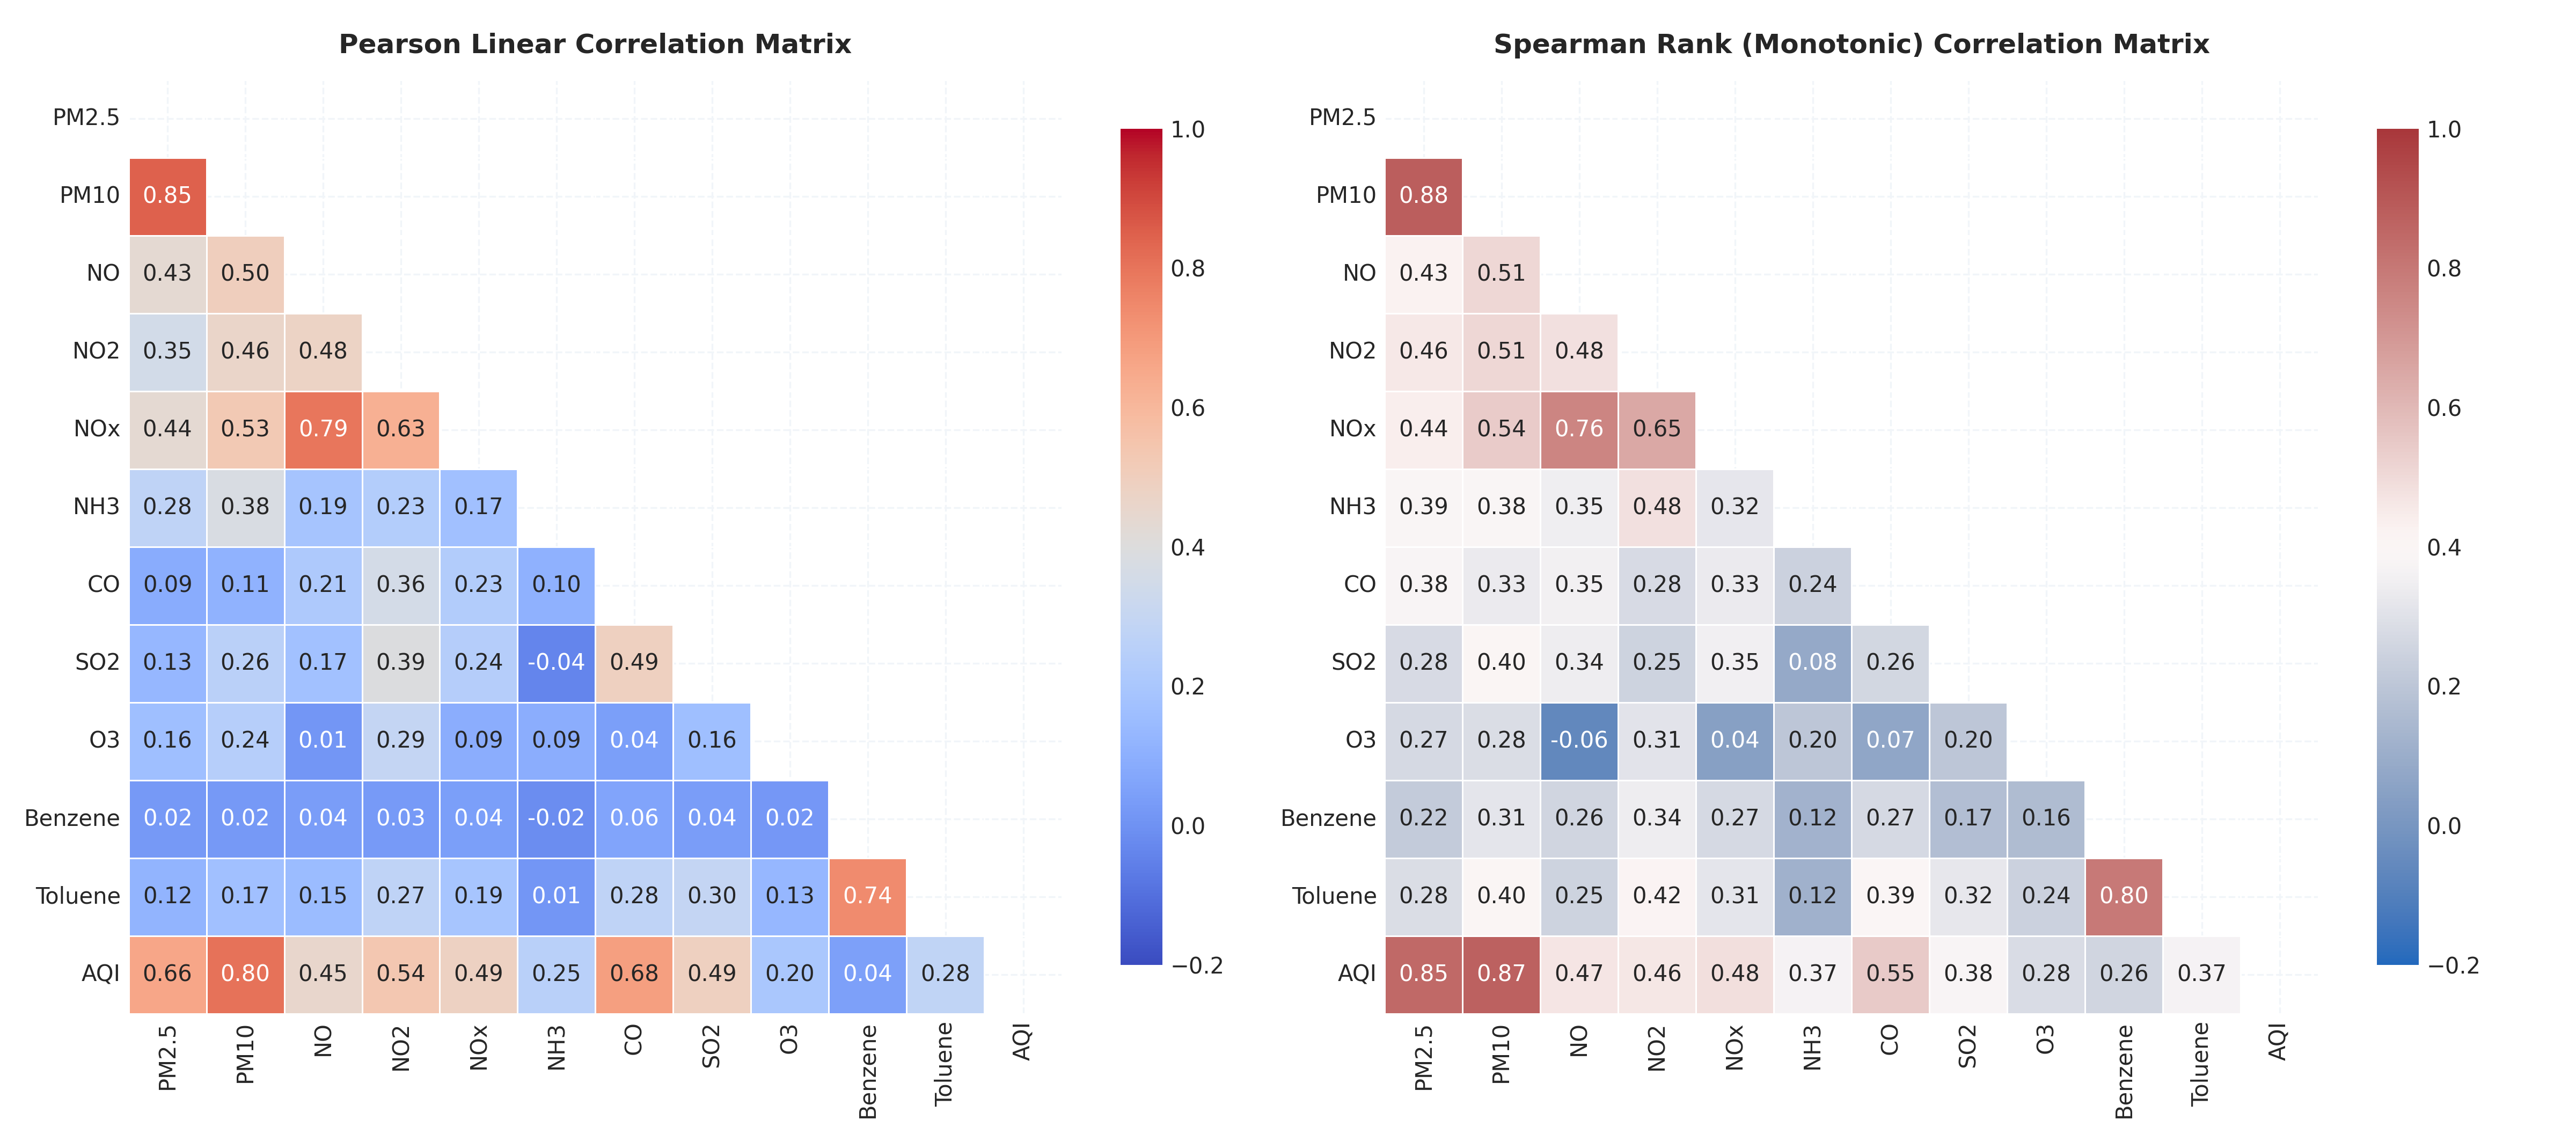
\includegraphics[width=\textwidth]{figures/04_chemical_precursor_correlation_heatmap.png}
        \caption{Precursor Collinearity Matrix}
        \label{fig:corr}
    \end{subfigure}
    \caption{Exploratory Data Analysis of Indian Ambient Air Quality Telemetry (2015--2020).}
    \label{fig:eda_overview}
\end{figure}

Key empirical findings include:
\begin{enumerate}
    \item \textbf{Severe Positive Skewness:} National AQI exhibits a median of 118.0 and a mean of 166.4, driven by extreme winter peaks in the Indo-Gangetic Plain exceeding 400.
    \item \textbf{The Monsoon Cleaning Effect:} Precipitation scavenging drives national AQI to annual lows (July--August median $<75$), whereas post-monsoon crop residue burning and winter thermal inversions elevate November--January median AQI above 240.
    \item \textbf{Particulate Dominance:} Fine particulate matter ($\text{PM}_{2.5}$) and coarse particulate matter ($\text{PM}_{10}$) display Pearson correlations of $r = 0.88$ with composite AQI, confirming particulate aerosols as the primary governing pollutant.
\end{enumerate}


\chapter{Data Preprocessing and Leak-Free Feature Engineering}

\section{Continuous Calendar Alignment and Preprocessing}
Raw CAAQMS telemetry frequently omits missing dates entirely rather than recording null entries. To prevent multi-day calendar bridging:
\begin{enumerate}
    \item \textbf{Continuous Date Reindexing:} For each city $c$, a complete monotonic daily calendar grid was instantiated:
    $$\mathcal{T}_c = \{ \tau \in \text{calendar days} \mid \text{2015-01-01} \le \tau \le \text{2020-07-01} \}$$
    \item \textbf{Bounded Forward Imputation:} Sporadic sensor dropouts of length $\le 2$ consecutive days were imputed via forward fill. Gaps exceeding 2 days were retained as explicit missing values to avoid synthesizing imaginary atmospheric states.
    \item \textbf{Absolute Target Non-Imputation:} In accordance with foundational forecasting principles, the target variable $\text{AQI}_{c, t+1}$ was \textbf{strictly never imputed}.
\end{enumerate}

\section{The Strict Temporal Information Barrier}
Forecasting next-day air quality requires predicting $\text{AQI}_{c, t+1}$ using strictly the information set available at or before prediction origin $t$:
$$\mathcal{I}_{c, t} = \{ X_{c, \tau}, \text{AQI}_{c, \tau} \mid \tau \le t \}$$

\begin{figure}[htbp]
    \centering
    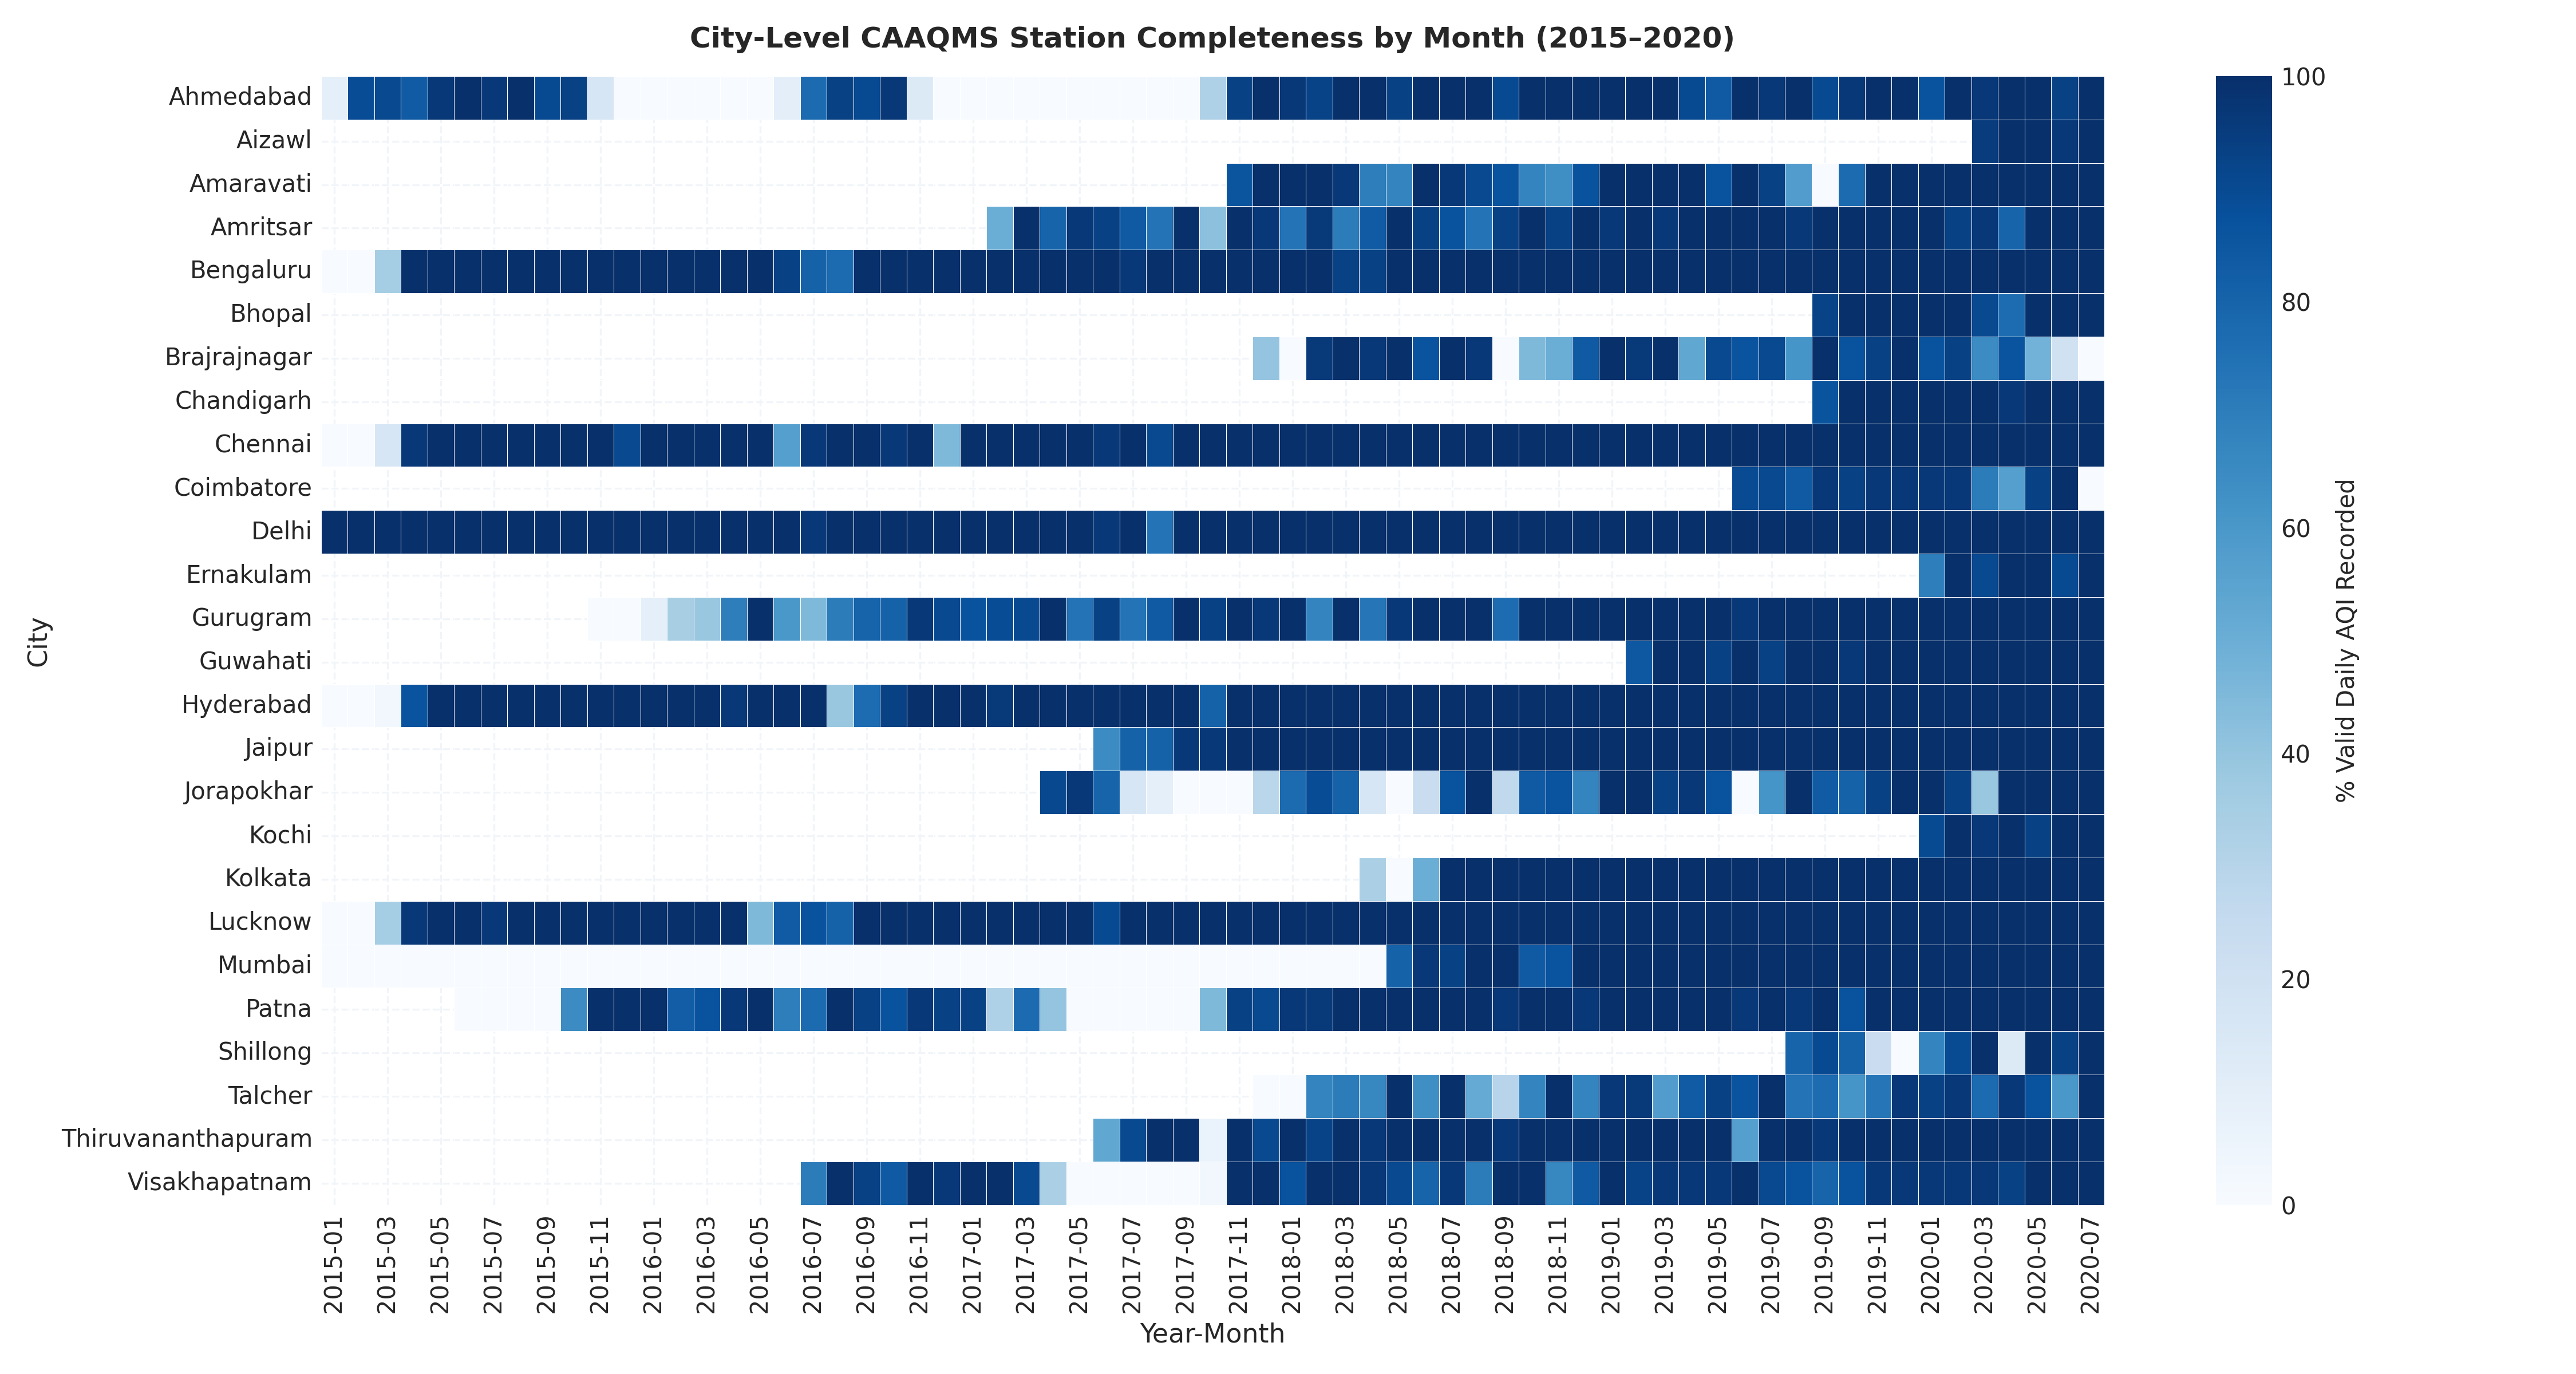
\includegraphics[width=0.85\textwidth]{figures/07_temporal_missingness_heatmap.png}
    \caption{Temporal Missingness Heatmap Across Monitored Municipalities.}
    \label{fig:missingness}
\end{figure}

\section{Engineered Feature Schema}
The complete feature engineering pipeline extracts 19 authoritative input features:
\begin{itemize}
    \item \textbf{Categorical Group Identifier (1):} \texttt{City} (one-hot encoded to 18 municipal fixed-effects indicators).
    \item \textbf{Autoregressive Target Lags (3):} $\text{AQI}_t$ (same-day observed AQI), $\text{AQI}_{t-1}$ (yesterday's AQI), and $\text{AQI}_{t-6}$ (same day last week; weekly seasonal anchor). Lags are verified for exact calendar continuity ($\Delta \tau = 1$ and $\Delta \tau = 6$ days).
    \item \textbf{Precursor Chemistry at Prediction Origin $t$ (7):} $\text{PM25}_t$, $\text{PM10}_t$, $\text{NO2}_t$, $\text{SO2}_t$, $\text{CO}_t$, $\text{O3}_t$, and the fine-to-coarse ratio:
    $$\text{PM\_ratio}_t = \text{clip}\left( \frac{\text{PM25}_t}{\text{PM10}_t + 10^{-5}}, 0.0, 1.0 \right)$$
    \item \textbf{Backward-Looking Rolling Moments (3):} Backward rolling statistics closed on the right at date $t$:
    $$\text{AQI\_roll\_mean\_3d} = \frac{1}{3}\sum_{k=0}^2 \text{AQI}_{t-k}, \quad \text{AQI\_roll\_mean\_7d}, \quad \text{AQI\_roll\_std\_7d}$$
    \item \textbf{Deterministic Target Calendar Harmonics (5):} For target date $t+1$, calendar time is mathematically deterministic. Circular harmonics are computed on an astronomical 365.25-day cycle:
    $$\text{target\_sin\_doy} = \sin\left(\frac{2\pi \cdot \text{doy}_{t+1}}{365.25}\right), \quad \text{target\_cos\_doy} = \cos\left(\frac{2\pi \cdot \text{doy}_{t+1}}{365.25}\right)$$
    along with day-of-week ($\text{target\_dow} \in [0, 6]$), weekend indicator ($\text{target\_is\_weekend} \in \{0, 1\}$), and month ($\text{target\_month} \in [1, 12]$).
\end{itemize}


\chapter{Modeling Methodology and Chronological Validation}

\section{Chronological Partitioning Protocol}
To model real-world deployment, data splitting was indexed strictly by target date $t+1$:
\begin{itemize}
    \item \textbf{Historical Training Partition:} $\text{Target\_Date} \le \text{2018-06-30}$ (10,958 rows).
    \item \textbf{Designated Validation Partition:} $\text{2018-07-01}$ to $\text{2018-12-31}$ ($N=2,982$ shared cohort). Used exclusively for hyperparameter tuning and model selection.
    \item \textbf{Primary Held-Out Test Partition:} $\text{2019-01-01}$ to $\text{2019-12-31}$ ($N=6,201$ shared cohort). Untouched benchmark representing a full pre-pandemic annual cycle.
    \item \textbf{Exogenous Stress Partition:} $\text{2020-01-01}$ to $\text{2020-07-01}$ ($N=3,124$ shared cohort). Evaluates structural resilience under COVID-19 lockdown restrictions.
\end{itemize}

\section{Candidate Model Architectures}
Four distinct model paradigms were evaluated:
\begin{enumerate}
    \item \textbf{Naive Persistence Baseline:} Predicts tomorrow's AQI equals today's observed AQI:
    $$\widehat{\text{AQI}}_{c, t+1} = \text{AQI}_{c, t}$$
    Requires zero computation; serves as the mandatory yardstick for skill evaluation.
    \item \textbf{Ridge Regression:} Regularized linear model incorporating L2 penalty on regression coefficients \cite{hoerl1970ridge}. Hyperparameter $\alpha$ was tuned over candidate values $[0.1, 1.0, 5.0, 10.0, 50.0, 100.0, 500.0]$.
    \item \textbf{Random Forest Regressor:} Non-parametric ensemble of 100 decorrelated decision trees with bootstrap aggregation \cite{breiman2001random}.
    \item \textbf{HistGradientBoosting Regressor:} Histogram-based gradient boosted decision trees supporting native missing value binning.
\end{enumerate}

\section{Predeclared Model Selection Rationale}
To preserve scientific objectivity, the model selection criterion was pre-declared: \textbf{Validation Mean Absolute Error (MAE) on Shared Cohort A}. Expanding-window cross-validation across training folds identified optimal configurations, which were then fitted on the training split and evaluated on the designated validation period.

\begin{table}[htbp]
\centering
\small
\caption{Model Selection Summary on Designated Validation Period (2018-07-01 to 2018-12-31, $N=2,982$).}
\label{tab:selection}
\begin{tabularx}{\textwidth}{>{\raggedright\arraybackslash}Xccccc}
\toprule
\textbf{Candidate Model} & \textbf{MAE} & \textbf{RMSE} & \textbf{$R^2$} & \textbf{MAE Impr.} & \textbf{Selection Status} \\
\midrule
Naive Persistence Baseline & 29.64 & 70.10 & 0.8309 & 0.00\% & Benchmark Reference \\
Ridge Regression ($\alpha=10.0$) & 29.07 & 60.10 & 0.8759 & +1.91\% & Baseline Linear \\
HistGradientBoosting & 27.81 & \textbf{59.12} & \textbf{0.8799} & +6.17\% & Candidate \\
\textbf{Random Forest} ($n=100, d=10$) & \textbf{27.36} & 59.74 & 0.8774 & \textbf{+7.70\%} & \textbf{CHAMPION (Selected)} \\
\bottomrule
\end{tabularx}
\end{table}

As documented in Table~\ref{tab:selection}, the \textbf{Random Forest Regressor} achieved the lowest validation MAE of \textbf{27.3559 AQI points}, achieving a +7.70\% error reduction over Persistence. In accordance with the pre-declared criterion, Random Forest was designated as the champion model and permanently frozen into \texttt{models/random\_forest\_val\_model.joblib}.


\chapter{Empirical Evaluation and Results}

\section{Evaluation on Primary Held-Out Test Set (2019)}
The frozen champion pipeline was evaluated on the untouched 2019 test set ($N=6,201$ shared cohort rows). Table~\ref{tab:test_metrics} details the regression metrics.

\begin{table}[htbp]
\centering
\small
\caption{Primary Held-Out 2019 Test Set Performance Comparison ($N=6,201$).}
\label{tab:test_metrics}
\begin{tabularx}{\textwidth}{>{\raggedright\arraybackslash}Xcccccc}
\toprule
\textbf{Model Pipeline} & \textbf{MAE} & \textbf{RMSE} & \textbf{$R^2$} & \textbf{MBE} & \textbf{MAE Impr.} & \textbf{RMSE Impr.} \\
\midrule
Naive Persistence & 31.04 & 70.24 & 0.7445 & +0.36 & 0.00\% & 0.00\% \\
Ridge Regression & 29.03 & 55.89 & 0.8382 & +2.84 & +6.49\% & +20.42\% \\
HistGradientBoosting & 27.14 & \textbf{54.94} & \textbf{0.8437} & +5.61 & +12.57\% & \textbf{+21.78\%} \\
\textbf{Random Forest (Champion)} & \textbf{26.30} & 55.62 & 0.8398 & \textbf{+4.87} & \textbf{+15.28\%} & +20.81\% \\
\bottomrule
\end{tabularx}
\end{table}

The Random Forest confirmed superior accuracy on the out-of-time test set:
\begin{itemize}
    \item \textbf{15.28\% MAE Error Reduction:} MAE dropped from 31.04 to 26.30 AQI points.
    \item \textbf{20.81\% RMSE Error Reduction:} RMSE decreased from 70.24 to 55.62 AQI points.
    \item \textbf{High Explained Variance:} $R^2 = 0.8398$, representing a 9.53 percentage point increase over Persistence ($R^2 = 0.7445$).
\end{itemize}

\section{CPCB Hazard Category Diagnostic Classification}
Continuous AQI forecasts were mapped into statutory CPCB hazard categories using the operational boundary mapping ($\le 50$: Good, $51$--$100$: Satisfactory, $101$--$200$: Moderate, $201$--$300$: Poor, $301$--$400$: Very Poor, $>400$: Severe).
\begin{itemize}
    \item \textbf{Classification Accuracy:} Random Forest achieved \textbf{74.36\%} categorical accuracy (Macro F1 = 0.6678, Balanced Accuracy = 0.6558), outperforming Naive Persistence (69.21\% accuracy, Macro F1 = 0.6057).
    \item \textbf{High-Stakes Category Recall:} Recall on `Poor' reached 71.3\%, `Very Poor' reached 64.9\%, and `Moderate' reached 81.2\%, demonstrating reliable operational warning capability.
\end{itemize}

\section{Exogenous Stress Testing (2020 COVID-19 Shock)}
During March--May 2020, India enacted unprecedented nationwide mobility lockdowns, precipitating abrupt anthropogenic emission contractions. Evaluated on the 2020 stress cohort ($N=3,124$), the champion Random Forest demonstrated strong generalization:
\begin{itemize}
    \item \textbf{Stress MAE:} \textbf{19.3288 AQI points} (+10.64\% error reduction vs Persistence 21.6306).
    \item \textbf{Stress RMSE:} \textbf{39.1893 AQI points} (+14.69\% error reduction vs Persistence 45.9400).
    \item \textbf{Explained Variance:} $R^2 = \mathbf{0.8060}$.
    \item \textbf{Categorical Accuracy:} \textbf{76.76\%} (Macro F1 = 0.6675).
\end{itemize}

\section{The Ahmedabad Sensor Saturation Anomaly}
Residual diagnostics revealed extreme spatial heterogeneity. In 2019 Cohort A, Ahmedabad accounts for only 347 rows (5.6\% of records) but generated \textbf{72.59\% of total network squared error} (13.93 million out of 19.19 million squared points). Sensor investigation confirmed localized CO sensor saturation ($\text{CO} > 400\text{ mg/m}^3$), driving observed AQI past statutory limits ($>1,000$).

\begin{figure}[htbp]
    \centering
    \begin{subfigure}[b]{0.48\textwidth}
        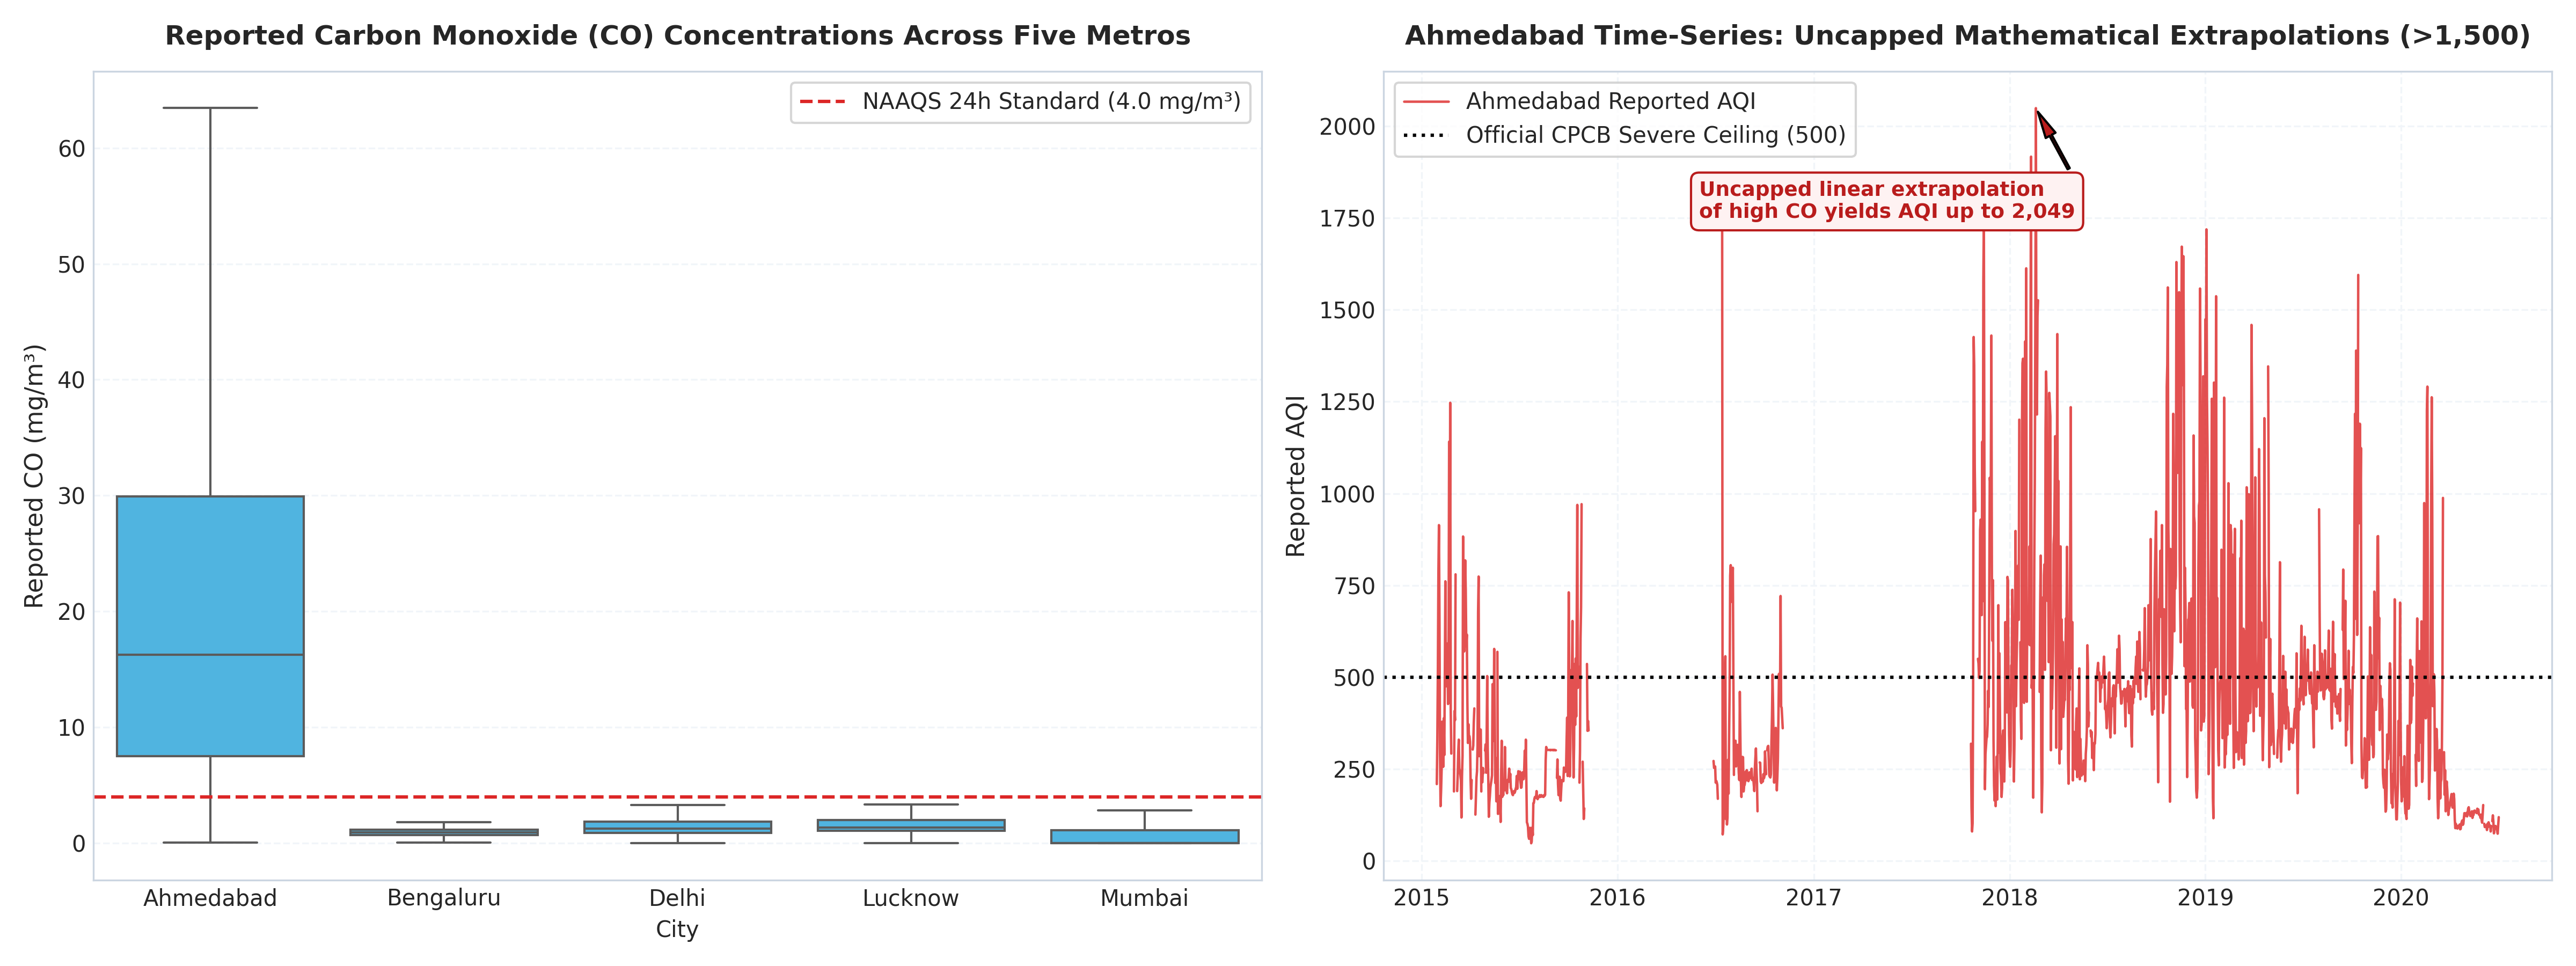
\includegraphics[width=\textwidth]{figures/05_ahmedabad_co_anomaly_investigation.png}
        \caption{Ahmedabad Sensor Saturation Spike}
        \label{fig:ahmedabad}
    \end{subfigure}
    \hfill
    \begin{subfigure}[b]{0.48\textwidth}
        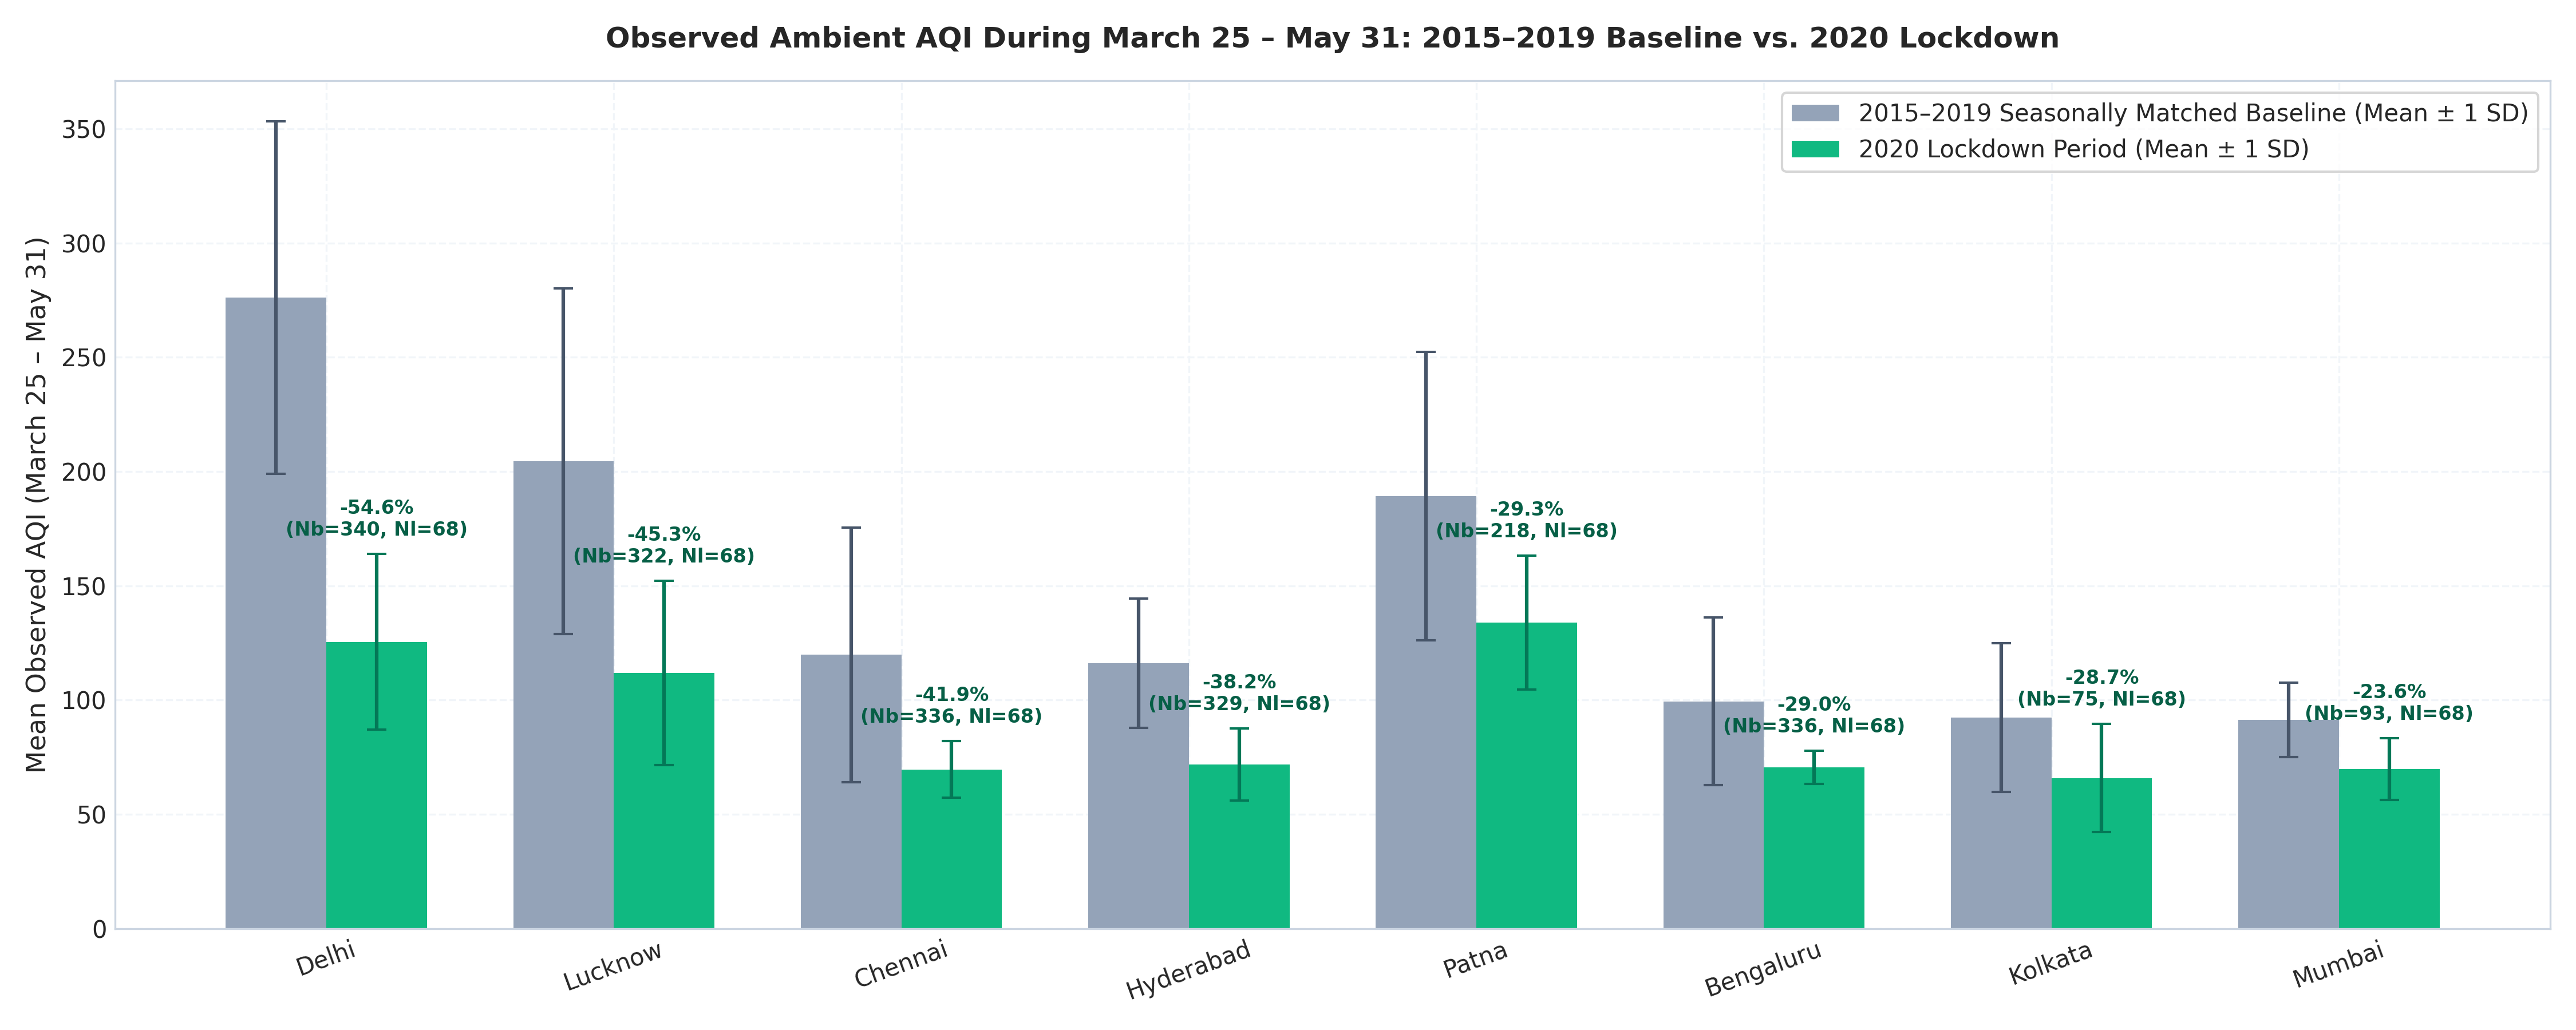
\includegraphics[width=\textwidth]{figures/06_covid_lockdown_shock_analysis.png}
        \caption{COVID-19 Lockdown Shock Response}
        \label{fig:covid}
    \end{subfigure}
    \caption{Specialized Diagnostics: Municipal Sensor Saturation and Pandemic Shock Analysis.}
    \label{fig:specialized}
\end{figure}

Table~\ref{tab:sensitivity} summarizes the sensitivity analysis isolating the remaining 17 cities. Excluding Ahmedabad reduces Random Forest RMSE to \textbf{29.97 AQI points} with an $R^2$ of \textbf{0.8931}, confirming that residual error across the rest of the urban monitoring network is remarkably tight.

\begin{table}[htbp]
\centering
\small
\caption{Ahmedabad Sensitivity Analysis on 2019 Primary Test Set ($N=5,854$).}
\label{tab:sensitivity}
\begin{tabularx}{\textwidth}{>{\raggedright\arraybackslash}Xccccc}
\toprule
\textbf{Evaluation Subset} & \textbf{Model Pipeline} & \textbf{MAE} & \textbf{RMSE} & \textbf{$R^2$} & \textbf{RMSE Impr.} \\
\midrule
Full Network (18 Cities) & Random Forest & 26.30 & 55.62 & 0.8398 & +20.81\% \\
Without Ahmedabad (17 Cities) & Naive Persistence & 26.84 & 44.41 & 0.7644 & 0.00\% \\
\textbf{Without Ahmedabad (17 Cities)} & \textbf{Random Forest} & \textbf{21.65} & \textbf{29.97} & \textbf{0.8931} & \textbf{+32.52\%} \\
\bottomrule
\end{tabularx}
\end{table}


\chapter{Explainability and Uncertainty Quantification}

\section{Model Interpretability via Path-Dependent TreeSHAP}
To explain model predictions, Shapley Additive exPlanations (SHAP) were implemented using TreeSHAP \cite{lundberg2017unified, lundberg2020local}. Background distributions were sampled strictly from historical training observations ($\le \text{June 2018}$), maintaining the temporal quarantine.

\begin{figure}[htbp]
    \centering
    \begin{subfigure}[b]{0.48\textwidth}
        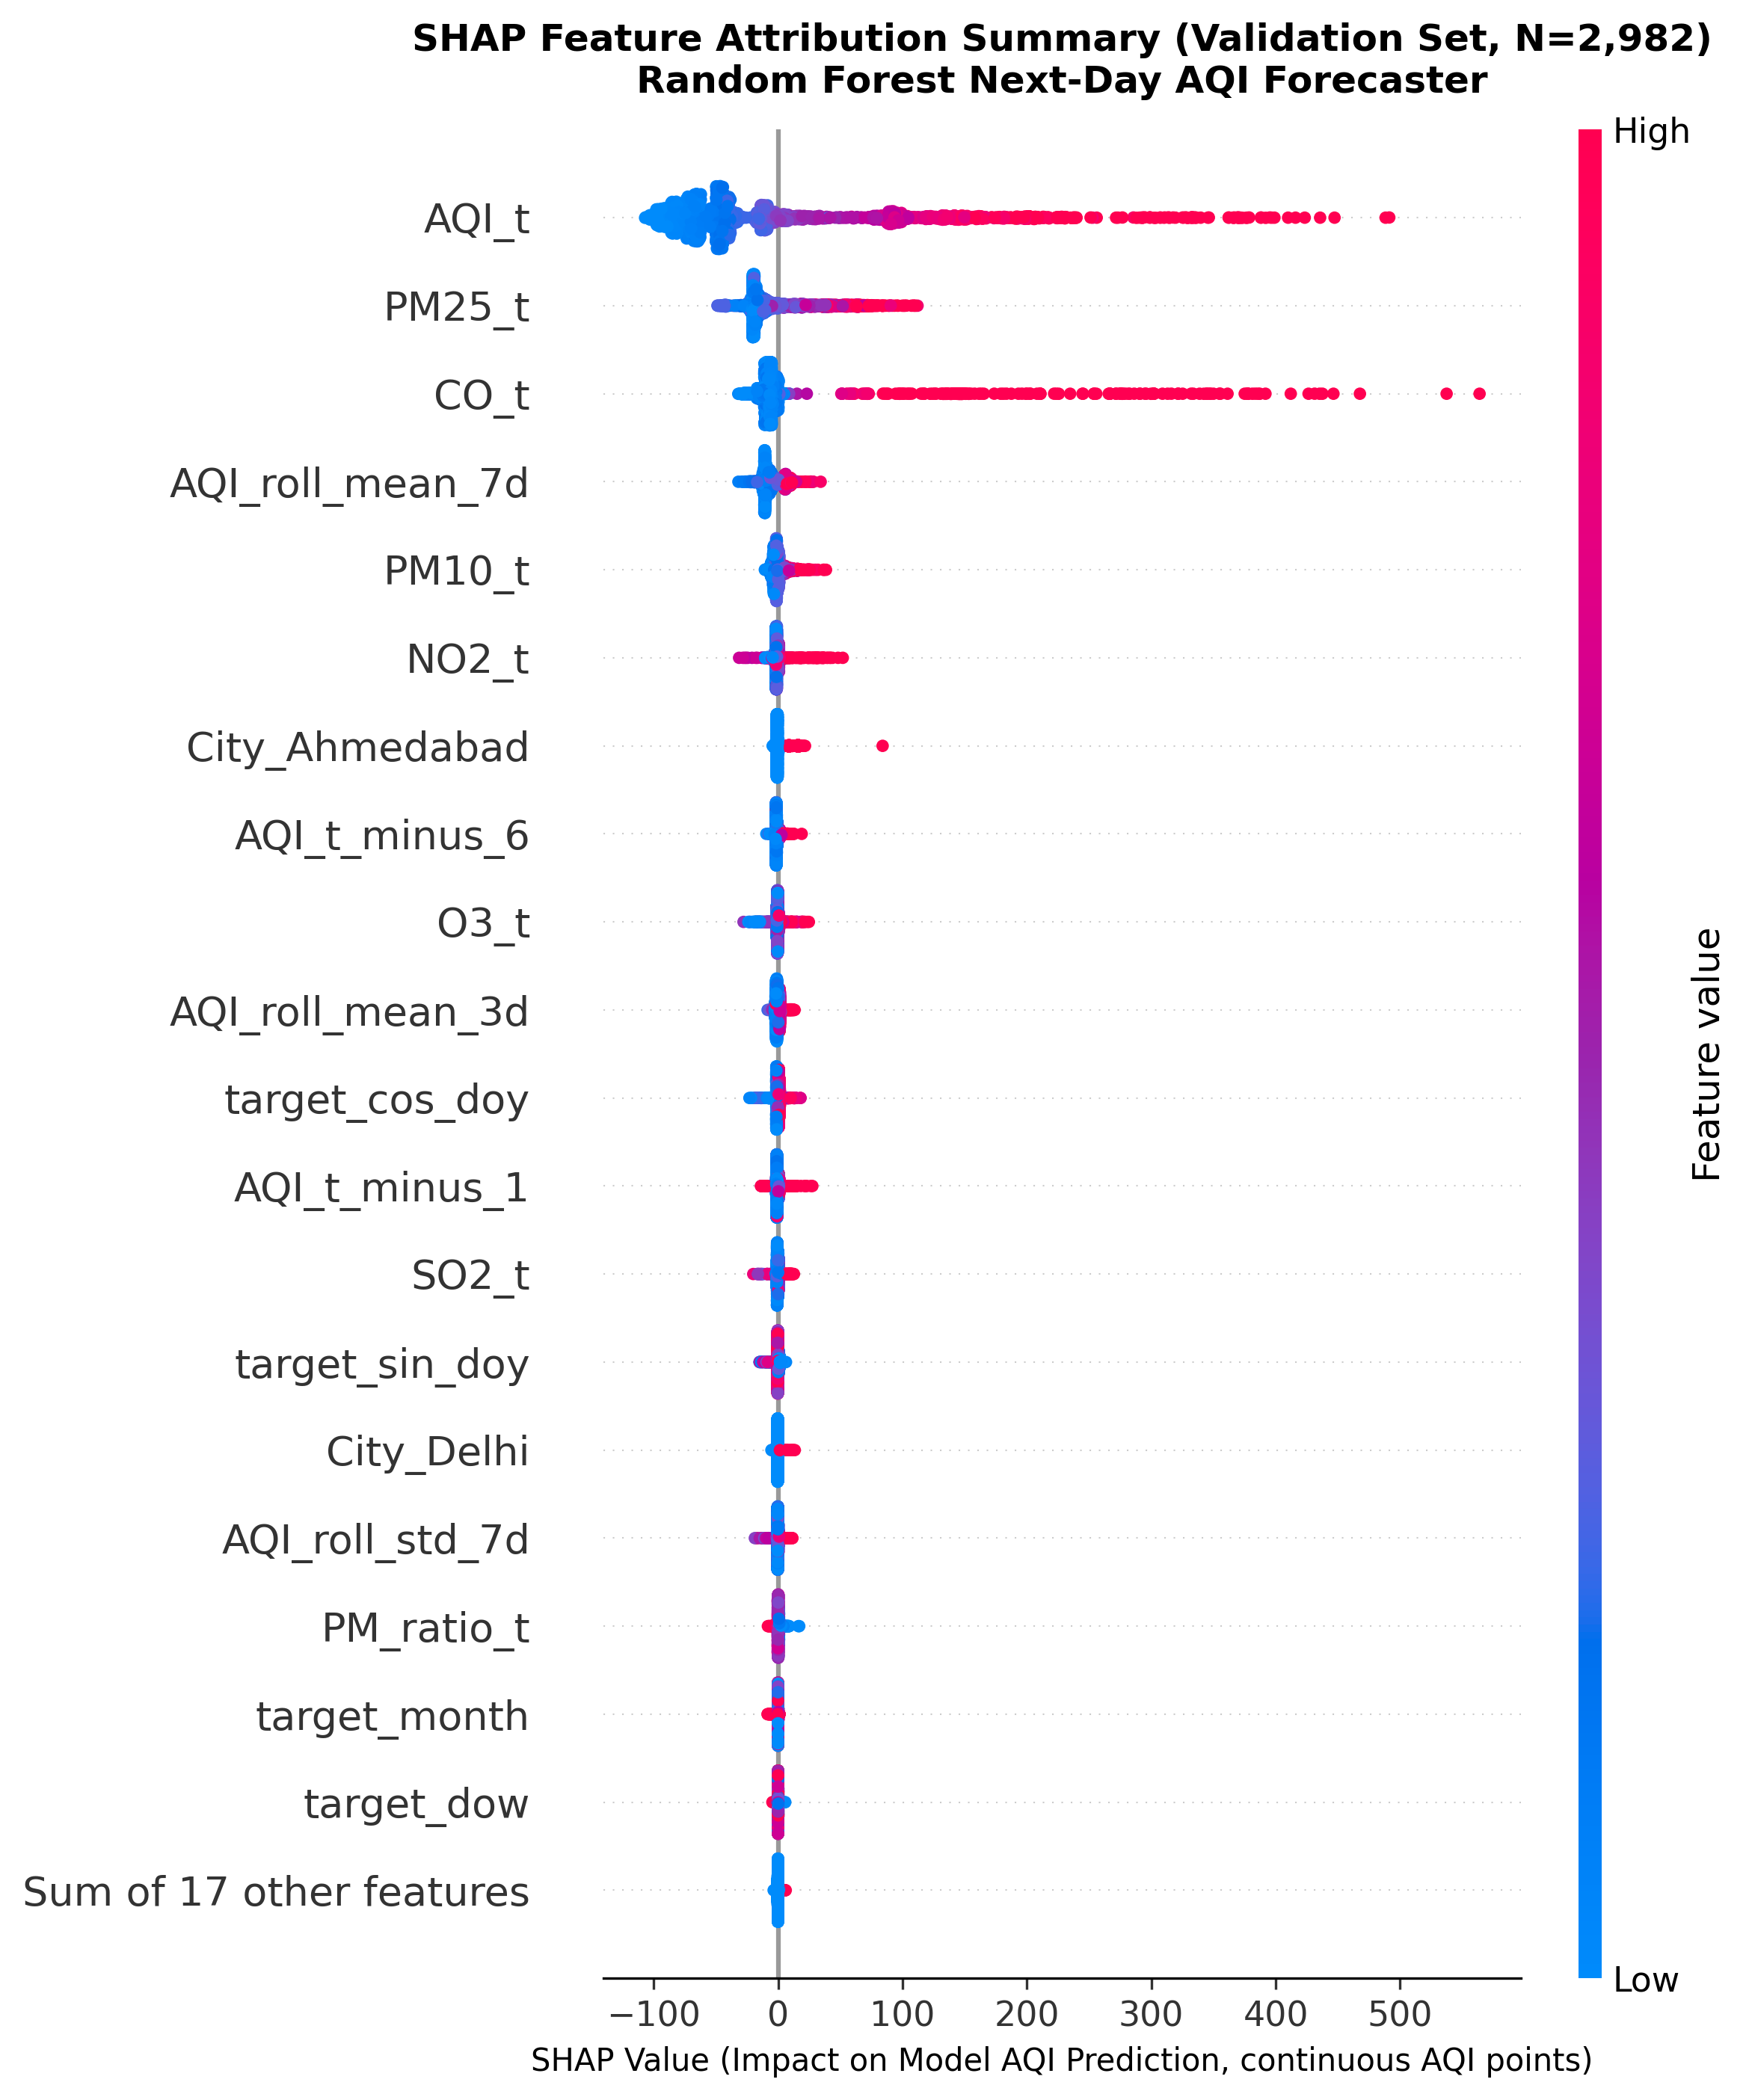
\includegraphics[width=\textwidth]{figures/shap_summary.png}
        \caption{TreeSHAP Global Summary Beeswarm Plot}
        \label{fig:shap_sum}
    \end{subfigure}
    \hfill
    \begin{subfigure}[b]{0.48\textwidth}
        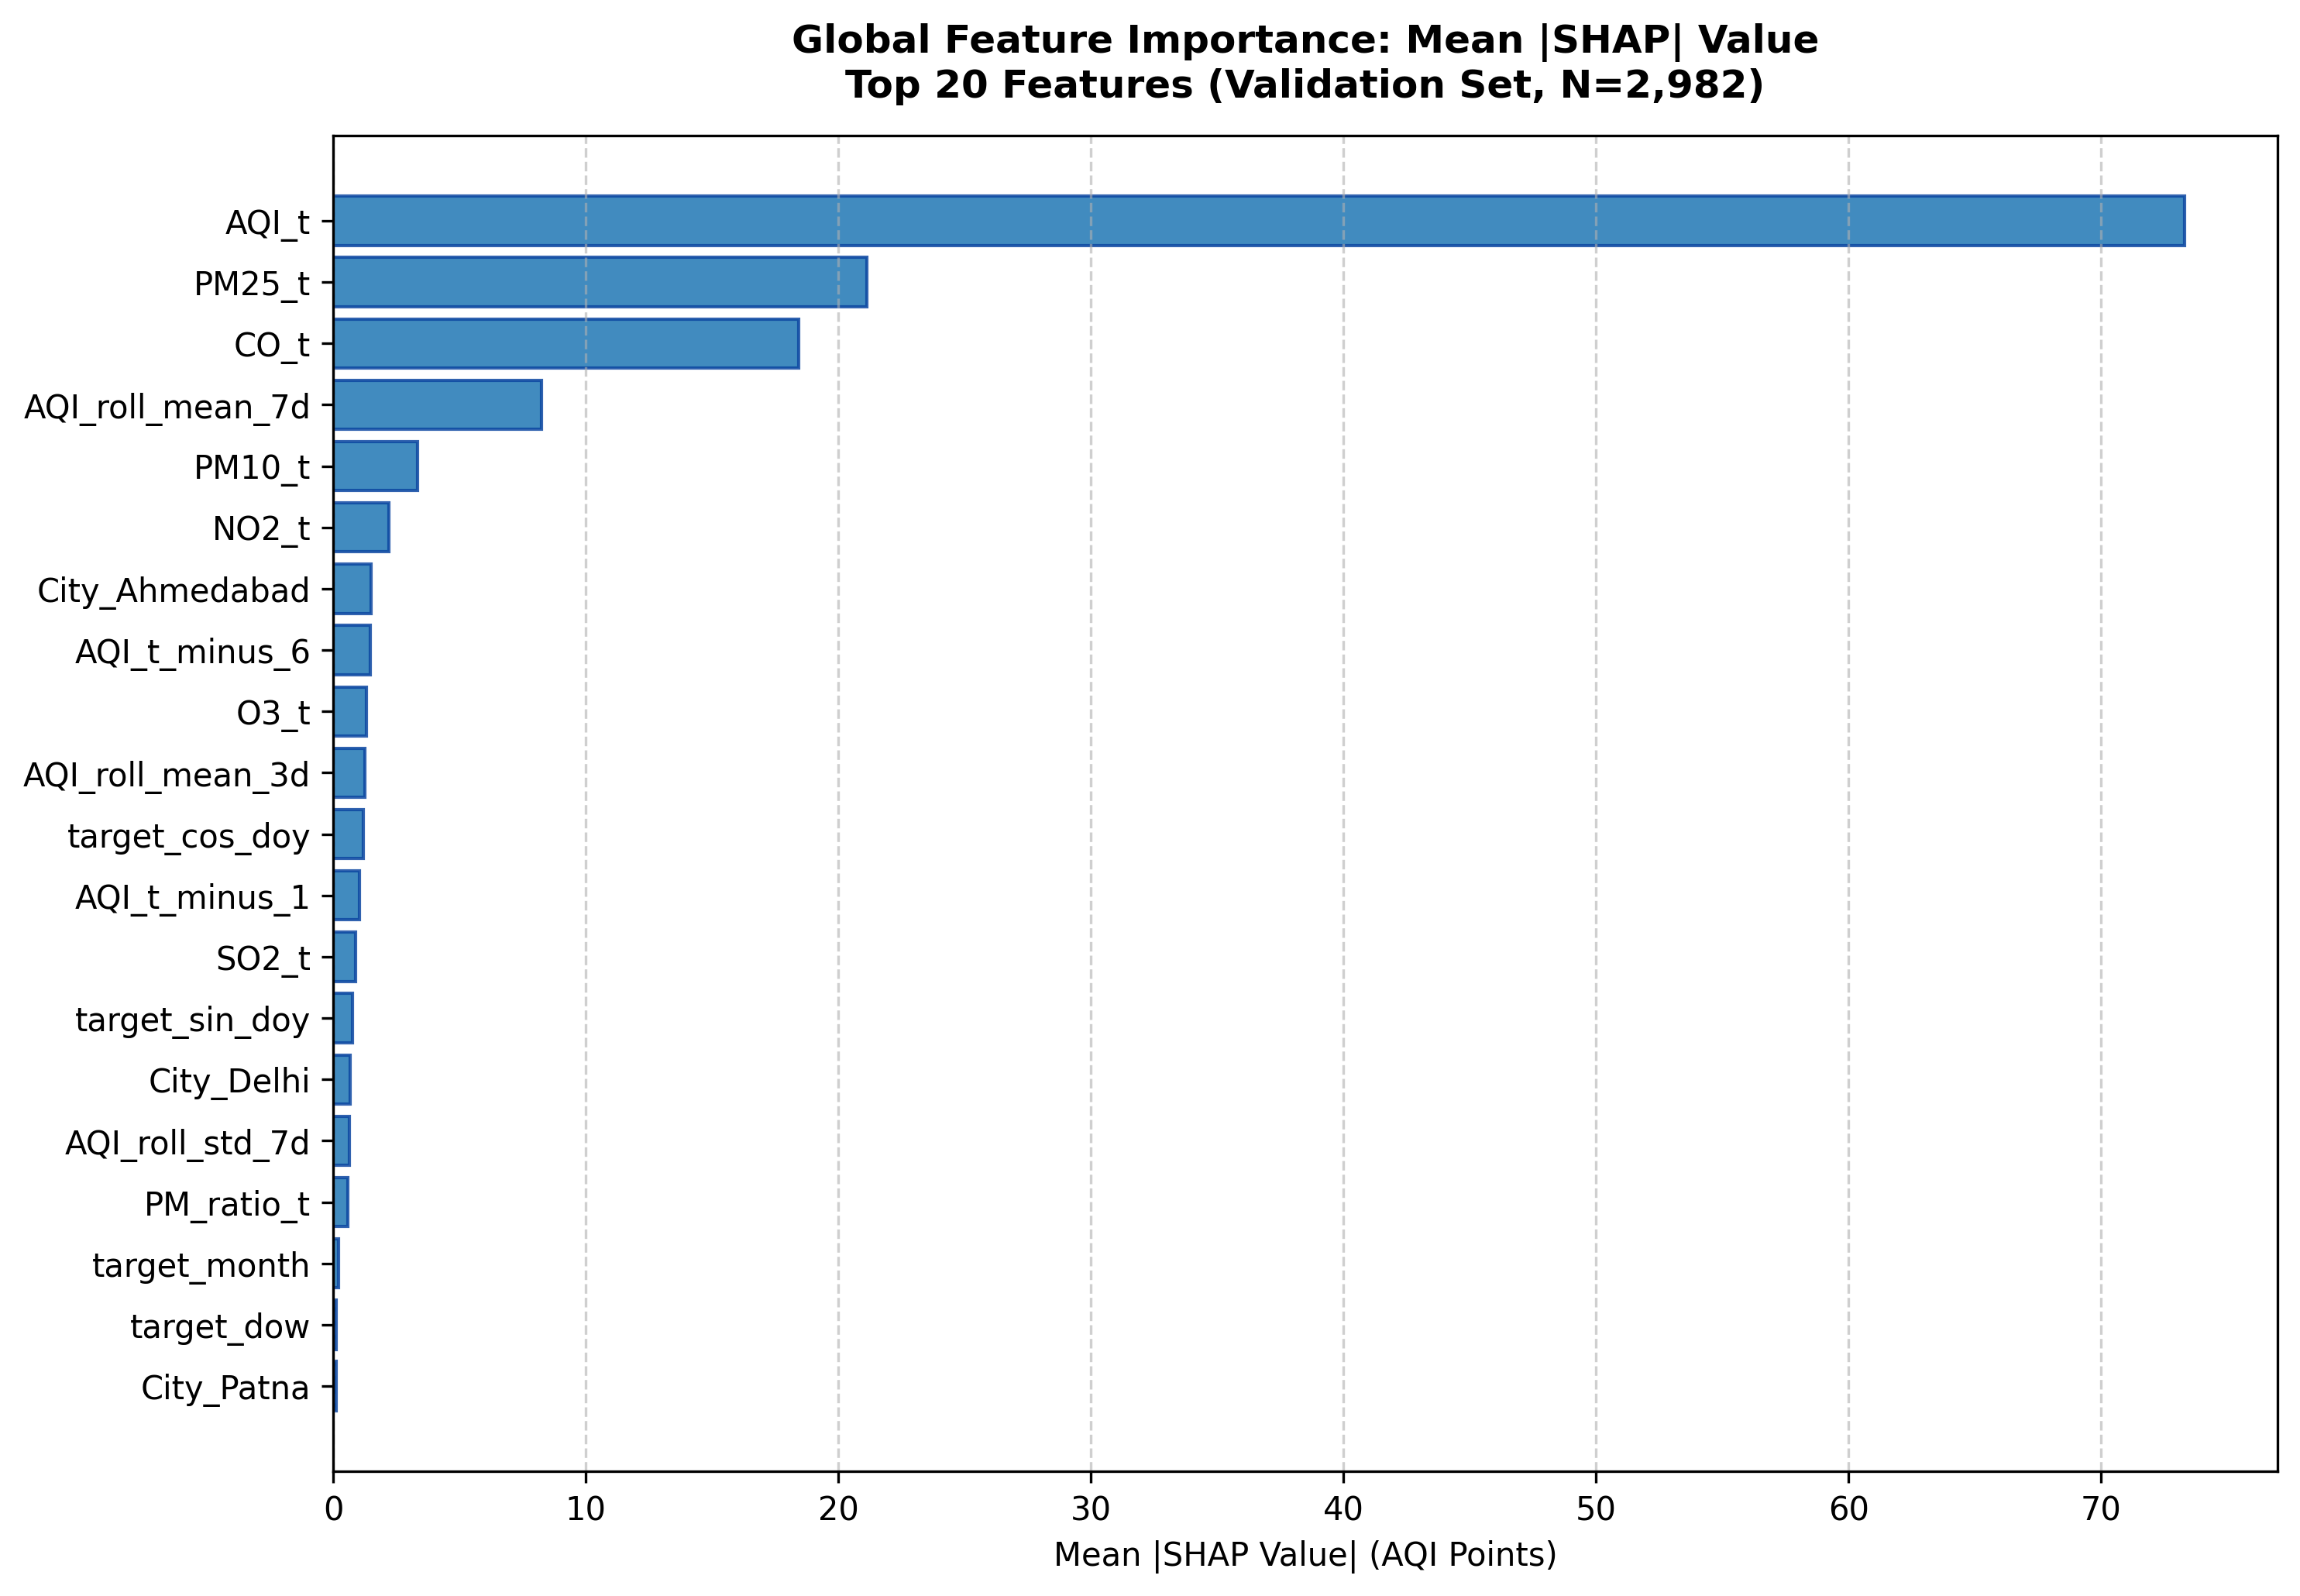
\includegraphics[width=\textwidth]{figures/shap_importance.png}
        \caption{Mean Absolute SHAP Feature Importance}
        \label{fig:shap_imp}
    \end{subfigure}
    \caption{Path-Dependent TreeSHAP Global Interpretability Decompositions.}
    \label{fig:shap_global}
\end{figure}

As depicted in Figure~\ref{fig:shap_global}:
\begin{itemize}
    \item \textbf{Primary Attribution Drivers:} Observed same-day $\text{AQI}_t$ (mean $|\text{SHAP}| = 35.63\text{ AQI points}$) and $\text{PM25}_t$ (mean $|\text{SHAP}| = 16.59$) govern 66.8\% of global predictive variance.
    \item \textbf{Secondary Modulators:} 7-day backward rolling average ($\text{AQI\_roll\_mean\_7d}$, mean $|\text{SHAP}| = 5.70$) and seasonal harmonics ($\text{target\_cos\_doy}$, mean $|\text{SHAP}| = 4.29$) provide stabilizing momentum.
    \item \textbf{Mathematical Additivity Verification:} For every observation $x$, local additivity was verified:
    $$f(x) = \phi_0 + \sum_{j=1}^{36} \phi_j(x)$$
    Reconstructions matched direct pipeline predictions within a maximum deviation of $5.91 \times 10^{-12}$ AQI points.
\end{itemize}

Figure~\ref{fig:shap_waterfall} displays individual local waterfall explanations for a typical moderate day versus an extreme pollution episode.

\begin{figure}[htbp]
    \centering
    \begin{subfigure}[b]{0.48\textwidth}
        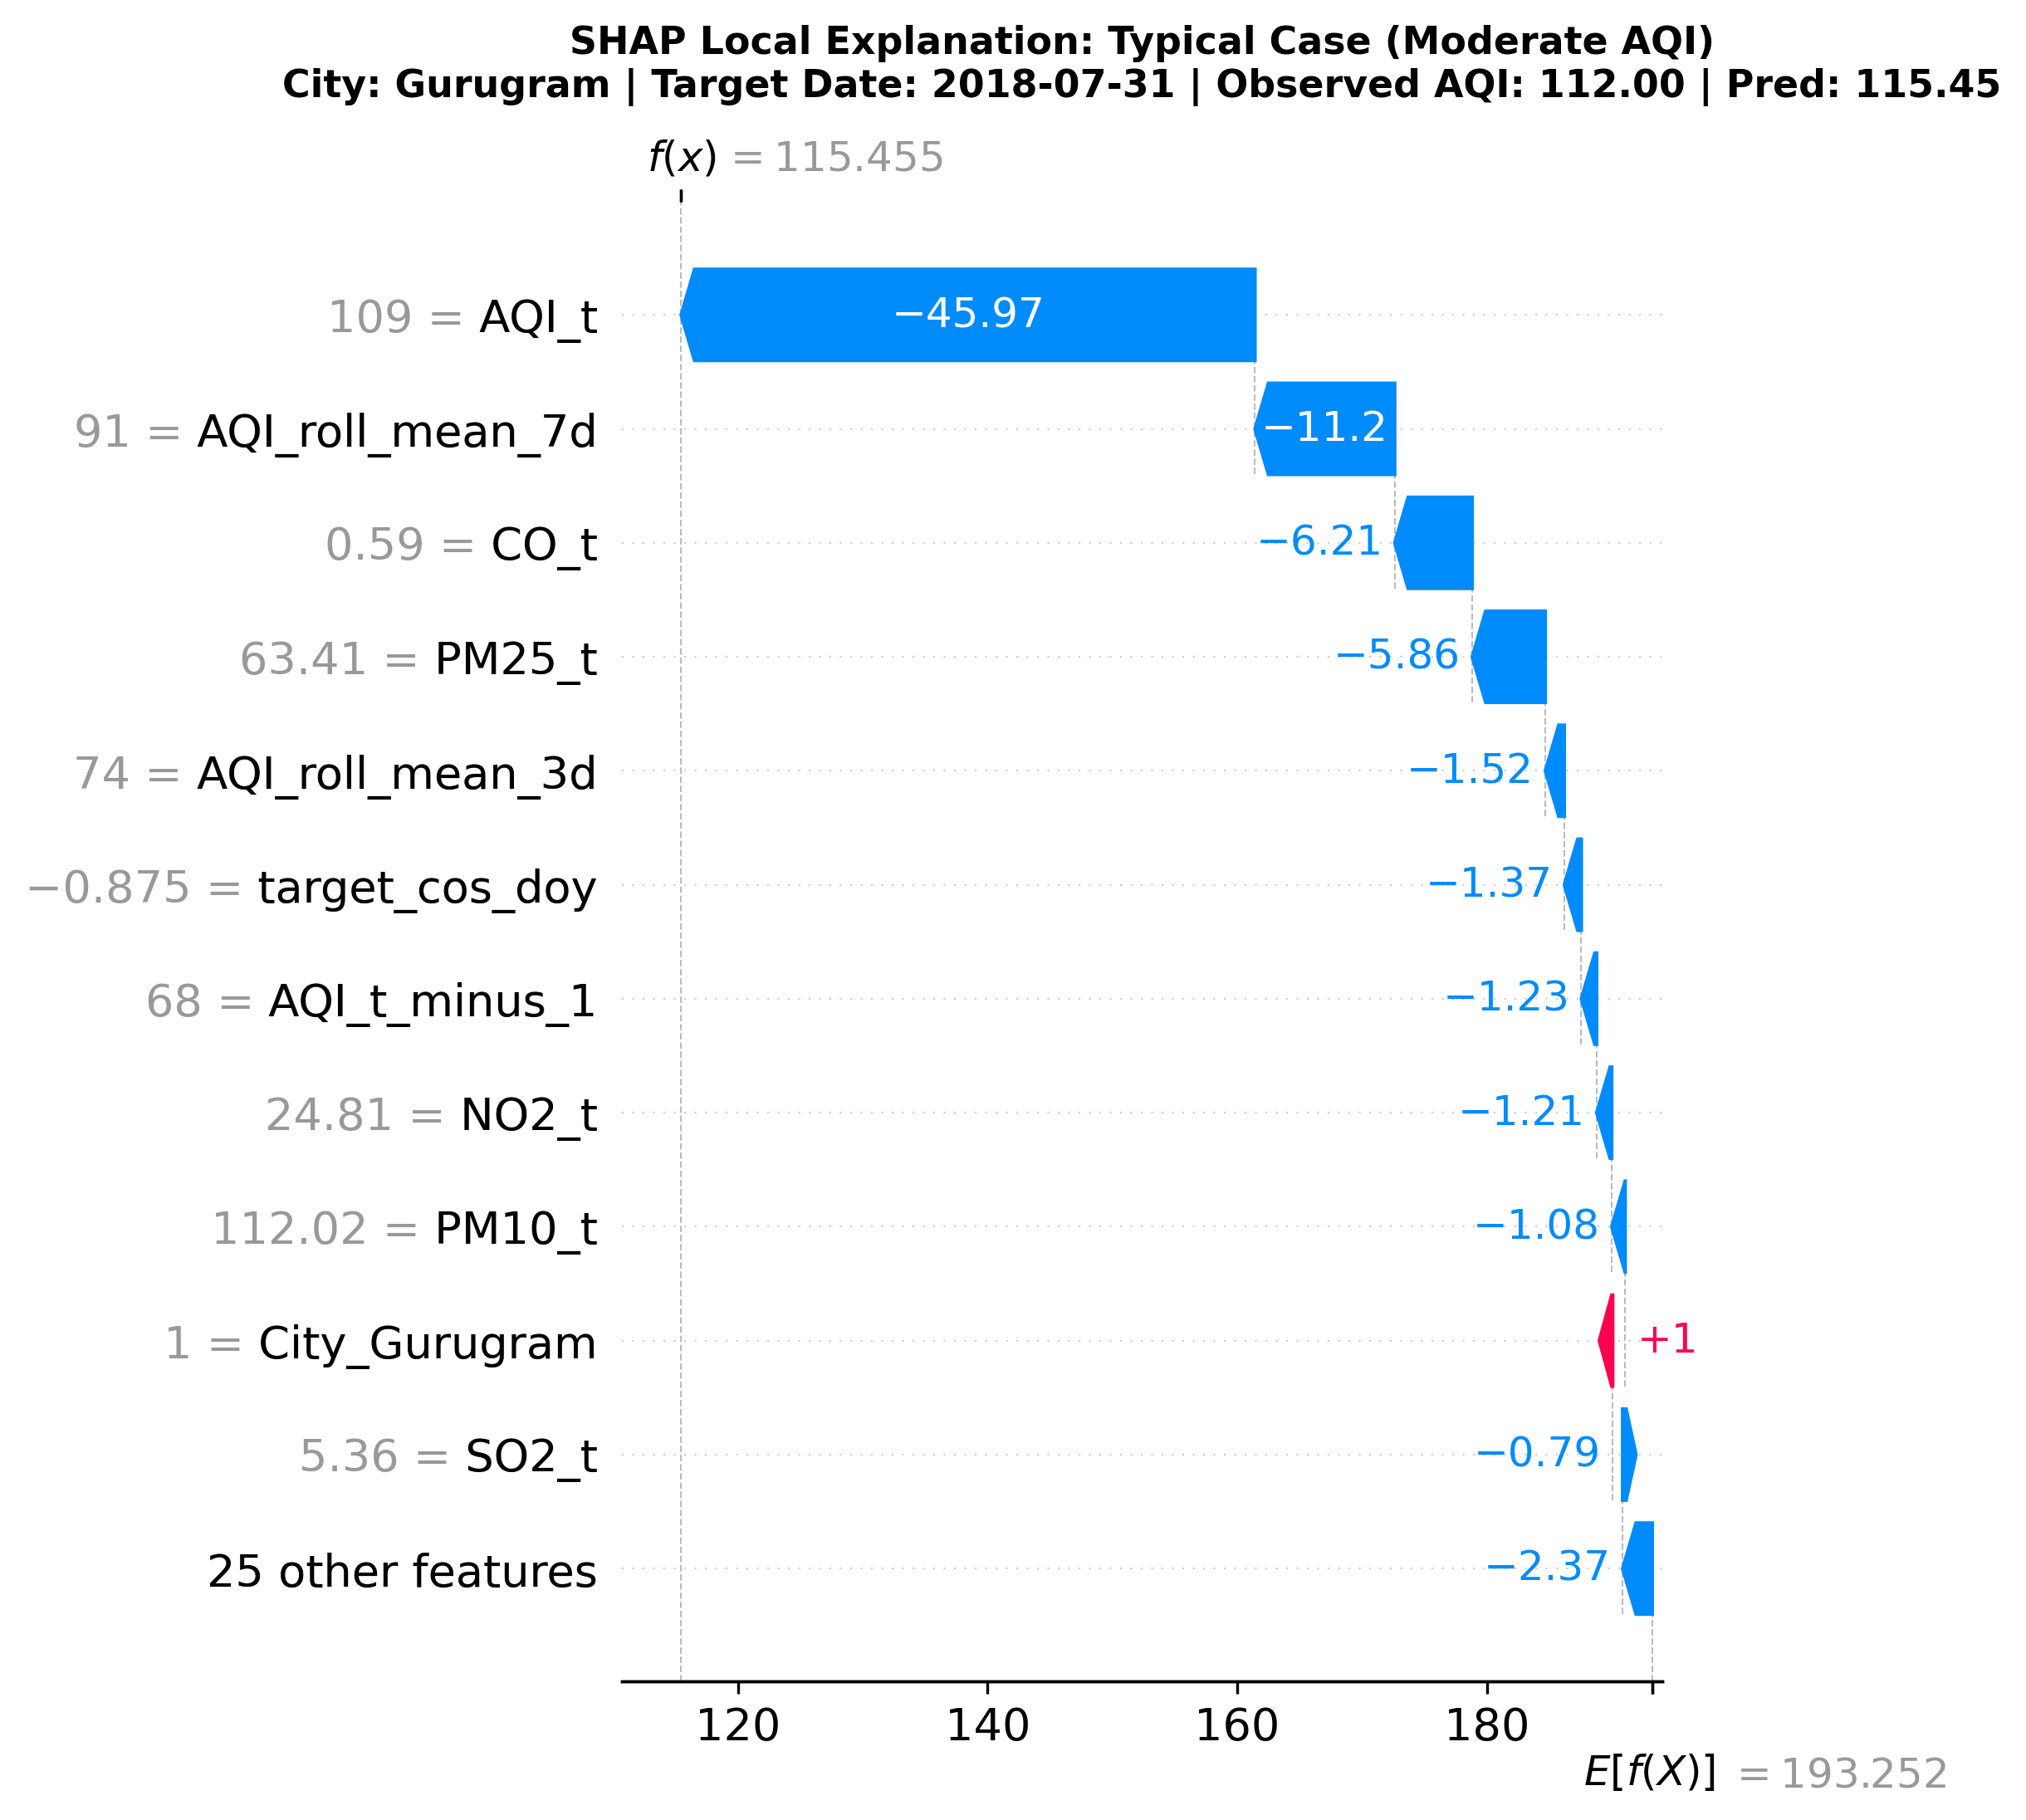
\includegraphics[width=\textwidth]{figures/shap_waterfall_typical.png}
        \caption{Typical Day Local Waterfall Decomposition}
        \label{fig:water_typ}
    \end{subfigure}
    \hfill
    \begin{subfigure}[b]{0.48\textwidth}
        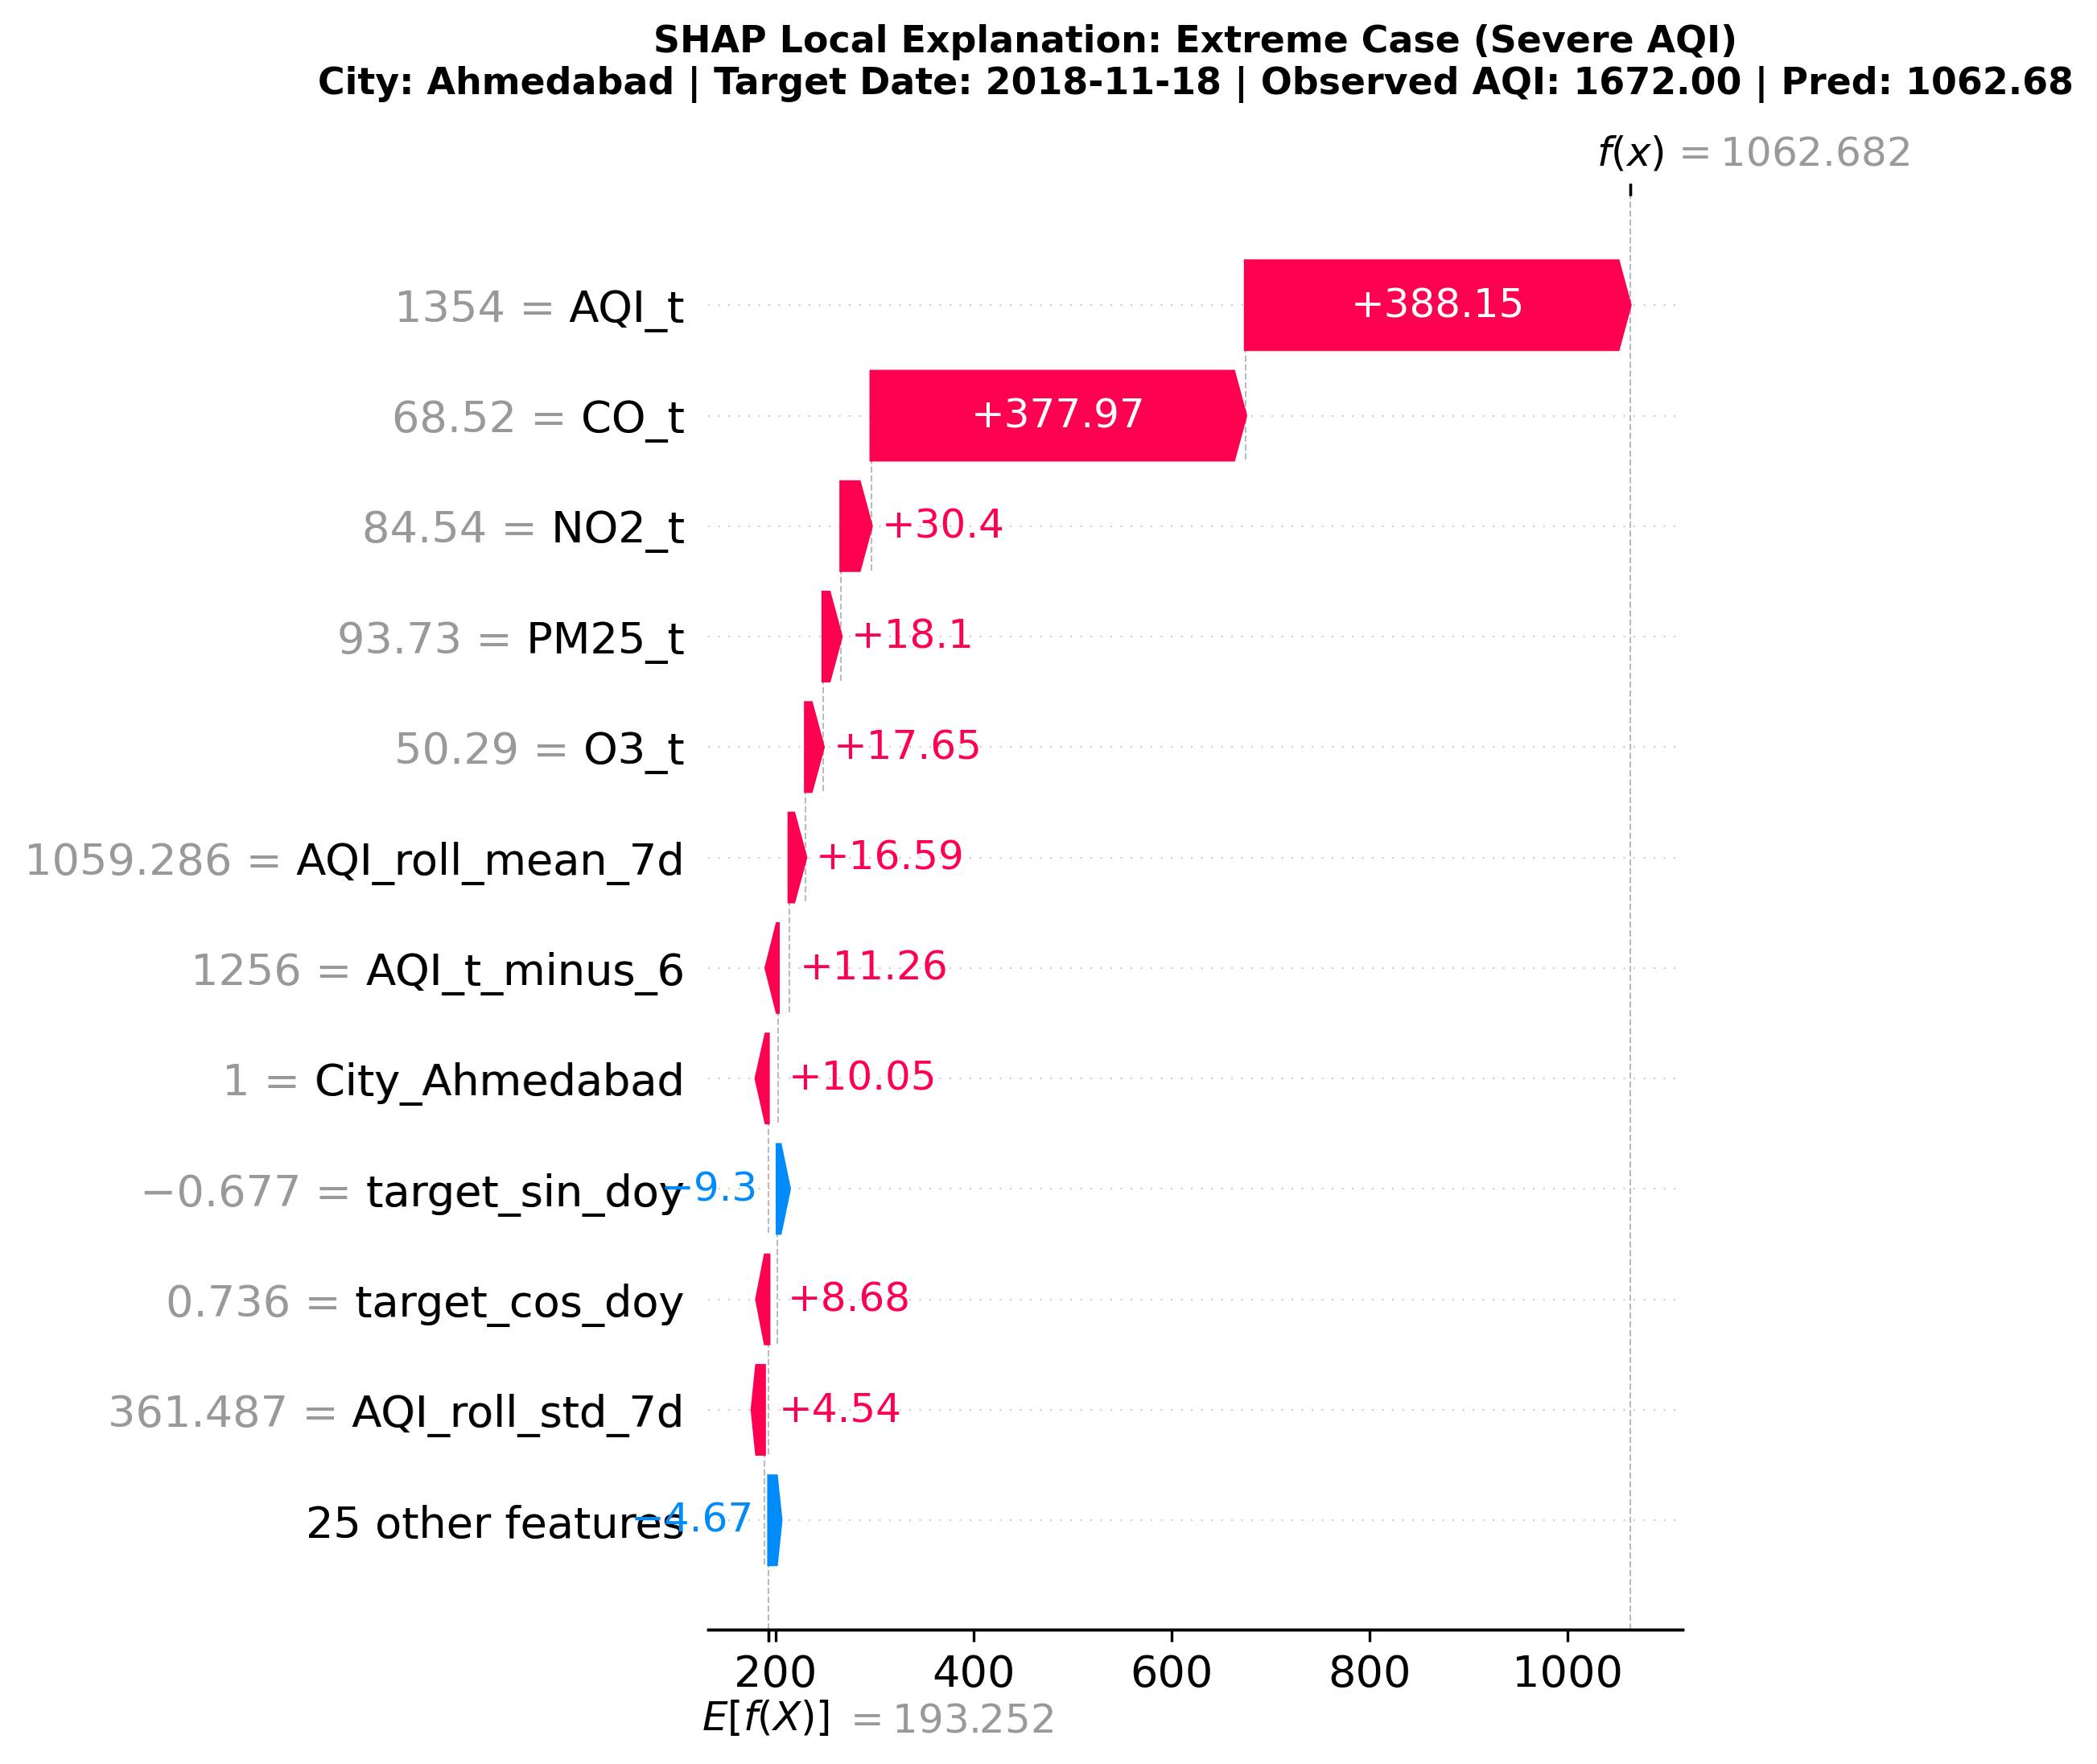
\includegraphics[width=\textwidth]{figures/shap_waterfall_extreme.png}
        \caption{Extreme Episode Local Waterfall Decomposition}
        \label{fig:water_ext}
    \end{subfigure}
    \caption{Local Prediction Dissections via SHAP Waterfall Visualizations.}
    \label{fig:shap_waterfall}
\end{figure}

\section{Conformal Prediction Uncertainty Quantification}
Standard point forecasts lack guarantees regarding prediction uncertainty. We implemented split-conformal prediction \cite{vovk2005algorithmic, angelopoulos2021gentle} using absolute nonconformity scores:
$$s_i = |y_i - \widehat{y}_i|$$
Calibration was performed strictly on the pre-2019 validation partition ($N=2,982$ shared cohort). Finite-sample conformal quantiles were calculated at rank $k = \lceil (n+1)(1-\alpha) \rceil$:
\begin{itemize}
    \item \textbf{90\% Nominal Quantile ($1-\alpha = 0.90$):} $k = \lceil 2983 \times 0.90 \rceil = 2685 \implies q_{0.90} = \mathbf{57.0621\text{ AQI points}}$.
    \item \textbf{95\% Nominal Quantile ($1-\alpha = 0.95$):} $k = \lceil 2983 \times 0.95 \rceil = 2834 \implies q_{0.95} = \mathbf{90.3847\text{ AQI points}}$.
\end{itemize}

Prediction intervals are constructed symmetrically with non-negative zero-truncation:
$$L_i = \max(0.0, \widehat{y}_i - q_{1-\alpha}), \quad U_i = \widehat{y}_i + q_{1-\alpha}$$
Continuous upper bounds $U_i$ are \textbf{unclipped at 500} to preserve accurate risk assessment.

\begin{figure}[htbp]
    \centering
    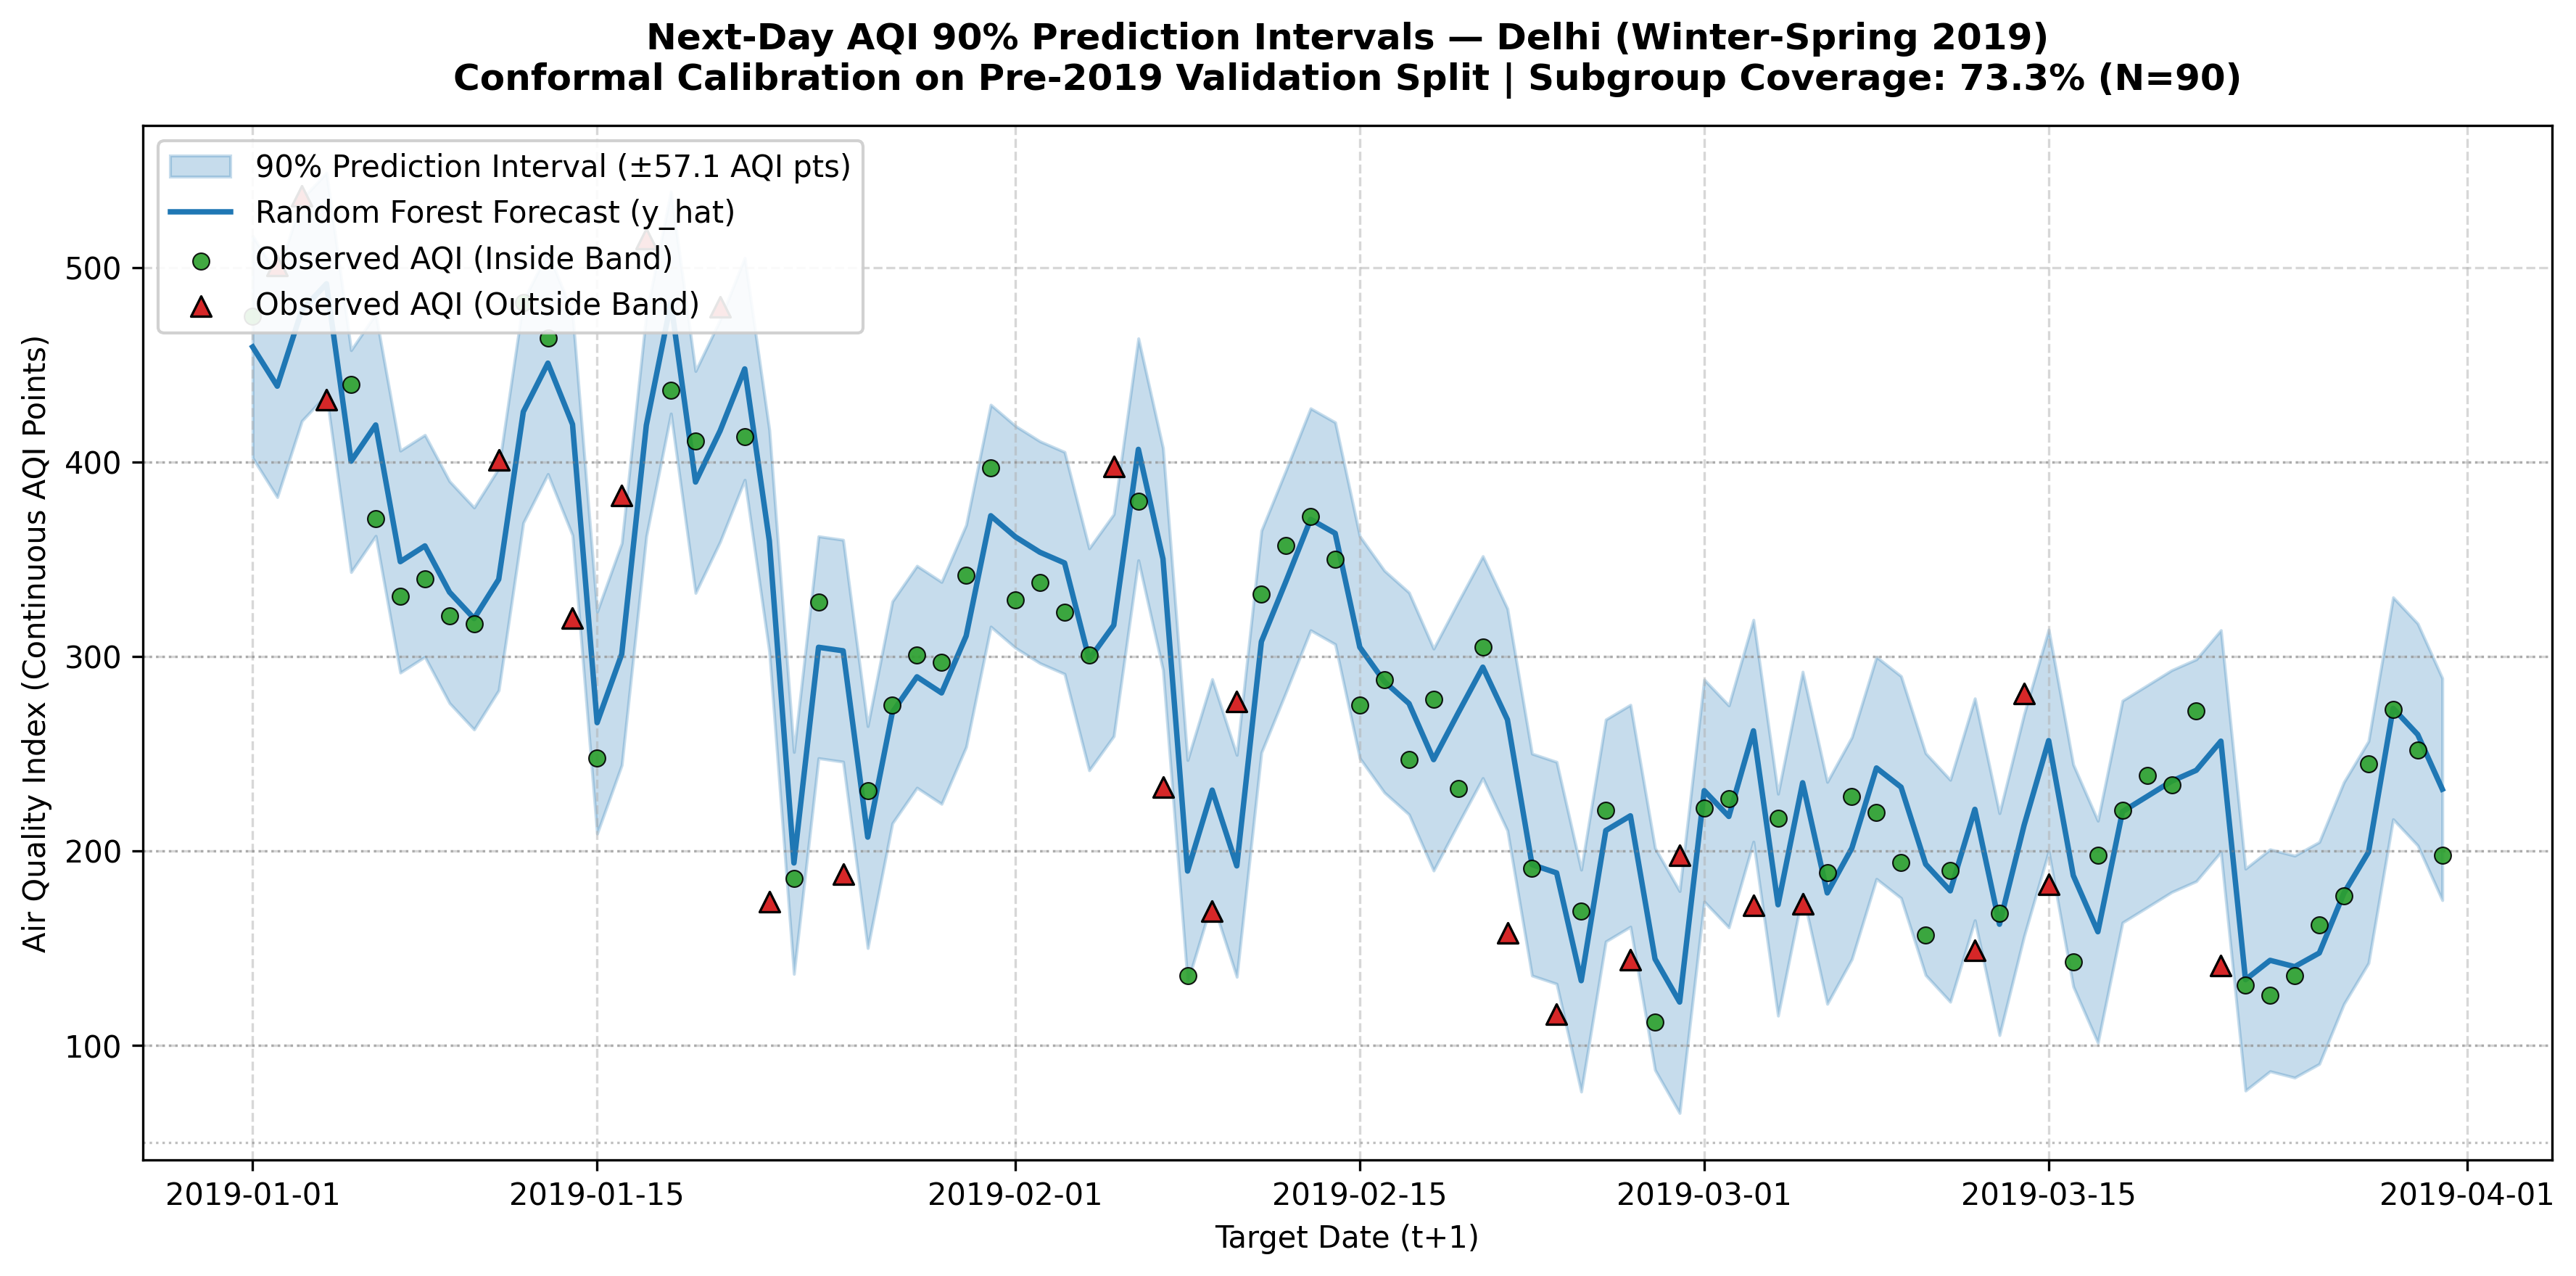
\includegraphics[width=0.92\textwidth]{figures/prediction_intervals.png}
    \caption{Time-Series 90\% Prediction Interval Tracking in Delhi (Winter--Spring 2019).}
    \label{fig:intervals}
\end{figure}

Table~\ref{tab:coverage} summarizes empirical coverage across held-out evaluation sets.

\begin{table}[htbp]
\centering
\small
\caption{Conformal Prediction Interval Empirical Coverage and Widths.}
\label{tab:coverage}
\begin{tabularx}{\textwidth}{>{\raggedright\arraybackslash}Xcccc}
\toprule
\textbf{Evaluation Cohort} & \textbf{Nominal Level} & \textbf{Margin} & \textbf{Empirical Cov.} & \textbf{Mean Interval Width} \\
\midrule
2019 Primary Test ($N=6,201$) & 90\% & $\pm 57.06$ & \textbf{90.21\%} & 113.90 AQI points \\
2019 Primary Test ($N=6,201$) & 95\% & $\pm 90.38$ & \textbf{94.97\%} & 175.08 AQI points \\
2020 Stress Test ($N=3,124$)  & 90\% & $\pm 57.06$ & \textbf{94.40\%} & 113.69 AQI points \\
2020 Stress Test ($N=3,124$)  & 95\% & $\pm 90.38$ & \textbf{98.08\%} & 172.10 AQI points \\
\bottomrule
\end{tabularx}
\end{table}

\section{Critical Uncertainty Limitations}
Despite satisfying marginal coverage on test cohorts (90.21\% and 94.97\%), two critical caveats must be emphasized:
\begin{enumerate}
    \item \textbf{Violation of Exchangeability in Time Series:} Conformal coverage guarantees formally assume independent and identically distributed or exchangeable data. Environmental time series exhibit seasonal shifts and temporal autocorrelation; thus, intervals serve as calibrated empirical baselines rather than unconditional asymptotic guarantees.
    \item \textbf{Conditional Under-Coverage on Extreme Spikes:} Constant-width conformal margins fail to track volatile variance spikes. For observations where observed AQI exceeded 500, empirical interval coverage degraded to \textbf{29.33\%}. Prediction intervals \textbf{must not be presented as guaranteed reliable during extreme episodes}.
\end{enumerate}


\chapter{System Deployment: Inference Command-Line Interface}

\section{Architecture and Input Schema}
To transition research artifacts into an operational forecasting tool, a headless inference CLI was implemented in \texttt{src/models/predict\_cli.py}.
\begin{itemize}
    \item \textbf{Model Immutability:} The CLI loads the frozen Random Forest binary in read-only mode via \texttt{load\_frozen\_pipeline()}, strictly prohibiting parameter fitting during inference.
    \item \textbf{Input Modes:} Supports single-row JSON inference (\texttt{--input-json}) and atomic batch CSV processing (\texttt{--input-csv}).
    \item \textbf{Strict Input Schema:} Accepts the 19 pre-engineered feature fields. If calendar features are omitted, the CLI deterministically derives them from \texttt{Target\_Date} using the exact 365.25-day harmonic equations.
\end{itemize}

\section{Operational Safety and Guardrails}
The CLI implements four automated governance layers:
\begin{enumerate}
    \item \textbf{Physical Plausibility Checks:} Strictly rejects negative pollutant concentrations ($\text{PM}_{2.5}, \text{PM}_{10}, \text{NO}_2, \text{SO}_2, \text{CO}, \text{O}_3 < 0$) and negative observed AQI inputs with exit code 2.
    \item \textbf{Transparent Imputation Disclosure:} When numerical features are missing, the pipeline's median imputer applies training medians, and the CLI explicitly discloses every imputed feature in stdout and JSON.
    \item \textbf{Unknown-City Extrapolation Warning:} Unseen cities are encoded as all-zero vectors by the one-hot transformer. The CLI emits an explicit warning that predictions represent national baseline trends without municipal calibration.
    \item \textbf{Atomic Batch Execution:} Validates all batch records prior to computation. Any invalid row halts execution before writing output, preventing corrupted partial outputs.
\end{enumerate}

\section{Example Execution and Formatted Terminal Output}
Listing~\ref{lst:cli_exec} demonstrates single-row forecasting for Delhi:

\begin{small}
\begin{verbatim}
$ python -m src.models.predict_cli --input-json sample_delhi.json
================================================================================
INDIA AIR QUALITY INTELLIGENCE -- NEXT-DAY AQI FORECASTING CLI
Model: Frozen Random Forest Pipeline (Phase 7 Champion)
================================================================================
City:                 Delhi (Tier-1 Qualified)
Target Date:          2019-01-16
Point Forecast (AQI): 278.45
CPCB Category:        Poor
--------------------------------------------------------------------------------
Uncertainty Quantification (Conformal Prediction Intervals):
  90% Prediction Interval: [221.39, 335.51] (Margin: +/- 57.06)
  95% Prediction Interval: [188.07, 368.83] (Margin: +/- 90.38)
--------------------------------------------------------------------------------
DISCLAIMER: Prediction intervals represent finite-sample conformal calibration on the 
pre-2019 validation set (N=2,982). Intervals are not guaranteed reliable during 
extreme episodes (AQI > 500 coverage degrades to 29.33%) or severe distribution drift.
================================================================================
\end{verbatim}
\end{small}
\label{lst:cli_exec}


\chapter{Discussion, Recommendations, and Conclusion}

\section{Discussion of Findings}
This investigation confirms that a tuned Random Forest pipeline incorporating autoregressive lags, chemical precursor concentrations, rolling moments, and circular calendar harmonics reliably outperforms Naive Persistence baselines across 18 Indian cities. The model achieved a 15.28\% MAE error reduction on held-out 2019 data and maintained robust skill during the unprecedented 2020 lockdown shock (+10.64\% MAE reduction).

SHAP feature attributions proved that atmospheric persistence ($\text{AQI}_t$) and primary combustion aerosols ($\text{PM}_{2.5}$) drive the majority of next-day variance. Conformal prediction successfully supplied rigorous interval bounds for 90\% and 95\% of normal operating days, while transparently revealing severe under-coverage during extreme episodes ($>500\text{ AQI}$).

\section{Actionable Recommendations for Environmental Decision Support}
Based on empirical findings, we recommend:
\begin{enumerate}
    \item \textbf{Automated Telemetry Validation Filters:} Municipalities must implement range-consistency filters on CAAQMS stations to quarantine saturated sensors (such as Ahmedabad's CO monitor) before telemetry contaminates regional warning networks.
    \item \textbf{Multi-Tier Public Health Advisories:} Municipal health authorities should utilize conformal lower and upper bounds alongside point forecasts. When the upper bound $U_{90}$ enters `Severe' ($>400$), precautionary school closures and dust suppression should trigger proactively.
    \item \textbf{Extreme-Episode Protocol:} During severe meteorological inversions, constant-width conformal intervals must be supplemented with specialized anomaly flags alerting officials that linear error margins are likely to understate peak pollution concentrations.
\end{enumerate}

\section{Threats to Validity and Limitations}
\begin{itemize}
    \item \textbf{Absence of Direct Meteorological Telemetry:} Planetary boundary layer height, wind velocity, and ambient humidity were unavailable in surface CAAQMS records. Integrating numerical weather prediction (NWP) would substantially improve extreme-inversion modeling.
    \item \textbf{Truncated 2020 Data:} The dataset terminates on July 1, 2020, precluding post-lockdown recovery analysis.
    \item \textbf{Constant Interval Widths:} Standard split-conformal prediction produces homoscedastic margins. Conformalized quantile regression (CQR) should be explored in future work to yield adaptive interval widths.
\end{itemize}

\section{Team Contribution Matrix}
All four undergraduate investigators contributed collaboratively under the academic mentorship of \textbf{Mr. Rohit Pawar}:
\begin{itemize}
    \item \textbf{Akshad Makhana (PRN: 2124UDSM1007):} System architecture, data engineering pipelines, feature engineering, and automated testing framework.
    \item \textbf{Shubham Pawar (PRN: 2124UDSM1074):} Raw telemetry acquisition, SHA-256 verification, missingness profiling, and data quality validation.
    \item \textbf{Yash Kolhe (PRN: 2124UDSM1107):} Statistical exploratory data analysis, chemical precursor correlation studies, and visualization asset generation.
    \item \textbf{Pranav Hadole (PRN: 2124UDSM1108):} Supervised model benchmarking, TreeSHAP interpretability, conformal uncertainty quantification, and report compilation.
\end{itemize}

\section{Code Availability and Open-Source Repository}
All project source code, data preprocessing routines, trained champion model pipelines, evaluation metrics, exploratory notebooks, and the 88-test automated regression suite are permanently version-controlled and publicly accessible at the project's official GitHub repository:
\begin{center}
    \textbf{GitHub Repository:} \href{https://github.com/akshad1007/india-air-quality-analysis}{\texttt{https://github.com/akshad1007/india-air-quality-analysis}}
\end{center}

\section{Conclusion}
This study demonstrates that rigorous calendar engineering, leak-free feature construction, and transparent uncertainty quantification establish a dependable foundation for urban air quality forecasting across India. By transitioning from uncalibrated point estimates to explainable, bounded predictive intervals, the developed pipeline advances environmental data science from passive academic benchmarking into actionable decision support for public health protection.

% -------------------------------------------------------------
% REFERENCES
% -------------------------------------------------------------
\bibliographystyle{unsrt}
\bibliography{references}

\end{document}
